% Canonical manuscript source: the LaTeX files in this directory.
% THESIS_DRAFT.md is a historical snapshot; the abstract is author-owned and hash-locked.
\documentclass[fontsize=13pt,paper=a4,DIV=calc,oneside,open=any,headings=normal,numbers=noenddot]{scrbook}
\usepackage{lmodern}
\usepackage{fontspec}
\IfFontExistsTF{Times New Roman}{\setmainfont{Times New Roman}}{\setmainfont{TeX Gyre Termes}}
\setsansfont{TeX Gyre Heros}
\setmonofont{Latin Modern Mono}[Scale=MatchLowercase]
\usepackage[a4paper,top=2.5cm,bottom=3cm,left=3cm,right=2cm,headheight=21pt]{geometry}
\usepackage{amsmath,amssymb,graphicx,booktabs,longtable,array}
\usepackage{float}
\usepackage{setspace,indentfirst,caption,scrlayer-scrpage,xurl}
\usepackage[unicode,hidelinks,breaklinks=true]{hyperref}
\usepackage{fvextra}
\usepackage{tikz}
\usetikzlibrary{calc}
\setstretch{1.3}
\setlength{\parindent}{1cm}
\setlength{\parskip}{6pt}
\setlength{\emergencystretch}{2em}
\setlength{\LTpre}{8pt plus 2pt minus 2pt}
\setlength{\LTpost}{8pt plus 2pt minus 2pt}
\setcounter{secnumdepth}{2}
\setcounter{tocdepth}{2}
\setkomafont{disposition}{\normalfont\bfseries}
\setkomafont{pageheadfoot}{\normalfont}
\setlength{\footheight}{21pt}
\RedeclareSectionCommand[beforeskip=0pt,afterskip=22pt]{chapter}
\RedeclareSectionCommand[beforeskip=15pt plus 3pt minus 2pt,afterskip=8pt plus 2pt,afterindent=true]{section}
\AddToHook{begindocument/end}{%
  \renewcommand{\chaptername}{Chương}%
  \renewcommand{\contentsname}{Mục lục}%
  \renewcommand{\listfigurename}{Danh mục hình}%
  \renewcommand{\listtablename}{Danh mục bảng}%
  \renewcommand{\bibname}{Tài liệu tham khảo}%
  \renewcommand{\appendixname}{Phụ lục}%
}
\captionsetup[figure]{name=Hình,position=bottom,labelfont=bf,labelsep=period}
\captionsetup[table]{name=Bảng,position=top,labelfont=bf,labelsep=period}
\clearpairofpagestyles
\cfoot*{\pagemark}
\newcommand{\thesistitle}{Nâng cao khả năng xử lý tác vụ chuỗi dài cho mô hình VLA trong điều khiển Robot}
\hypersetup{pdftitle={\thesistitle},pdfauthor={Lưu Quang Linh},pdfsubject={Khóa luận về bộ nhớ sự kiện thị giác cho mô hình VLA},pdflang={vi-VN}}

\begin{document}
\pagenumbering{Roman}
% Metadata confirmed by the student; no signature is generated.
\newcommand{\coverframe}{%
  \begin{tikzpicture}[remember picture,overlay]
    \draw[line width=2pt] ($(current page.north west)+(2cm,-2cm)$)
      rectangle ($(current page.south east)+(-1.5cm,1.8cm)$);
    \draw[line width=.7pt] ($(current page.north west)+(2.15cm,-2.15cm)$)
      rectangle ($(current page.south east)+(-1.65cm,1.95cm)$);
  \end{tikzpicture}}
\begin{titlepage}
\thispagestyle{empty}\coverframe
\begin{center}
{\bfseries ĐẠI HỌC QUỐC GIA HÀ NỘI\\TRƯỜNG ĐẠI HỌC CÔNG NGHỆ\par}
\vspace{1cm}
\includegraphics[width=2.4cm]{assets/UET.png}\par
\vspace{1cm}
{\Large\bfseries LƯU QUANG LINH\par}
\vspace{1.5cm}
{\fontsize{18}{25}\selectfont\bfseries\MakeUppercase{\thesistitle}\par}
\vspace{1.8cm}
{\bfseries KHÓA LUẬN TỐT NGHIỆP ĐẠI HỌC HỆ CHÍNH QUY\par}
\vspace{.3cm}
{\bfseries Ngành: Trí tuệ nhân tạo\par}
\vfill
{\bfseries HÀ NỘI - 2026\par}
\end{center}
\end{titlepage}

\begin{titlepage}
\thispagestyle{empty}\coverframe
\begin{center}
{\bfseries ĐẠI HỌC QUỐC GIA HÀ NỘI\\TRƯỜNG ĐẠI HỌC CÔNG NGHỆ\par}
\vspace{1.3cm}
{\Large\bfseries LƯU QUANG LINH\par}
\vspace{1.3cm}
{\fontsize{18}{25}\selectfont\bfseries\MakeUppercase{\thesistitle}\par}
\vspace{1.6cm}
{\bfseries KHÓA LUẬN TỐT NGHIỆP ĐẠI HỌC HỆ CHÍNH QUY\par}
{\bfseries Ngành: Trí tuệ nhân tạo\par}
\vspace{1.8cm}
\begin{minipage}{.92\textwidth}
\textbf{Cán bộ hướng dẫn:} PGS.TS. Nguyễn Việt Hà\par
\textbf{Cán bộ đồng hướng dẫn:} PGS.TS. Hoàng Văn Xiêm\par
\end{minipage}
\vfill
{\bfseries HÀ NỘI - 2026\par}
\end{center}
\end{titlepage}

\pagestyle{empty}
\chapter*{Lời cảm ơn}
\thispagestyle{empty}

Lời đầu tiên, em xin được gửi lời cảm ơn chân thành và sâu sắc nhất tới \textbf{PGS. TS. Nguyễn Việt Hà} và \textbf{PGS. TS. Hoàng Văn Xiêm}, những người thầy đã luôn tận tâm định hướng nghiên cứu, trực tiếp chỉ bảo và tạo mọi điều kiện thuận lợi nhất cho em trong suốt quá trình thực hiện khóa luận tốt nghiệp này.

Em cũng xin gửi lời cảm ơn tới các thầy cô giáo tại Trường Đại học Công nghệ, Đại học Quốc gia Hà Nội, đặc biệt là cô \textbf{Nguyễn Thị Thùy Linh} đã truyền đạt những kiến thức quý báu và nền tảng chuyên môn vững chắc cho em trong suốt những năm học tập và nghiên cứu vừa qua của em.

Cuối cùng, em xin gửi lời cảm ơn sâu sắc tới gia đình và bạn bè, những người đã luôn ở bên động viên, ủng hộ và là chỗ dựa tinh thần vững chắc để em hoàn thành tốt khóa luận này.

\vspace{1.5cm}
\begin{flushright}
\begin{tabular}{c}
\textit{Hà Nội, tháng 11 năm 2026} \\
\textbf{Sinh viên thực hiện} \\
\vspace{2cm} \\
\textbf{Lưu Quang Linh}
\end{tabular}
\end{flushright}

% Generated from THESIS_DRAFT.md.
\chapter*{Tóm tắt}
\thispagestyle{empty}

Trong thao tác robot chuỗi dài, các quan sát hiện tại có thể không cho biết một chu kỳ đã hoàn tất hay chưa, dù quyết định tiếp theo phụ thuộc vào lịch sử tương tác. Khóa luận xây dựng bộ nhớ sự kiện có bằng chứng cho mô hình thị giác - ngôn ngữ - hành động (VLA), nhằm lưu giữ các mốc tiến độ đã được xác nhận và cung cấp chúng qua một bản tóm tắt ngôn ngữ gọn nhẹ phù hợp với giới hạn ngữ cảnh.

Mỗi sự kiện được gắn với bằng chứng quan sát và thời điểm khả dụng; khi lịch sử thiếu hoặc bị gián đoạn, hệ thống giữ trạng thái chưa xác định thay vì suy diễn tiến độ. Khóa luận chứng minh hai tính chất hình thức trong phạm vi các giả định đã nêu: bộ nhớ sự kiện chỉ thay đổi khi có chuyển tiếp hợp lệ, và nội dung cung cấp cho chính sách tại thời điểm hiện tại chỉ phụ thuộc dữ liệu đã có đến thời điểm đó. Bản ghi được chiếu thành văn bản và dùng để thích ứng các chính sách VLA.

Đánh giá thực nghiệm của nghiên cứu bao gồm phân tích tiền huấn luyện, can thiệp vào prompt chỉ dẫn hành động, đo đạc điều khiển vòng kín, kiểm chứng cơ chế dừng ngoại vi dựa trên bộ nhớ và đo mức duy trì hiệu năng trên tác vụ gốc sau tinh chỉnh. Kết quả xác nhận cơ chế truy vấn theo sự kiện vận hành được và cho thấy mô hình phản ứng với nội dung bộ nhớ trong các trường hợp khảo sát. Dù lợi ích trực tiếp qua lời nhắc còn hạn chế đối với tỷ lệ thành công nội tại, việc khai thác bằng chứng bộ nhớ cho cơ chế dừng ngoại vi bước đầu giúp chuyển hóa các chu kỳ thao tác hoàn thành thành thành công toàn phần. Mức duy trì hiệu năng sau tinh chỉnh cũng khác biệt rõ rệt giữa hai mô hình nền. Các kết quả này làm rõ khả năng vận hành và giới hạn thực nghiệm của phương pháp, đồng thời đặt ra nhu cầu xác nhận trên tập trạng thái rộng hơn với nhiều ngẫu nhiên hơn.

\textbf{Từ khóa:} Mô hình thị giác - ngôn ngữ - hành động, Tác vụ long-horizon, Bộ nhớ sự kiện, Quan sát một phần, Thao tác robot.


\chapter*{Lời cam đoan}
\thispagestyle{empty}

Tôi xin cam đoan đây là công trình nghiên cứu của chính tôi dưới sự hướng dẫn khoa học của PGS. TS. Nguyễn Việt Hà và PGS. TS. Hoàng Văn Xiêm. 

Các kết quả nghiên cứu, phân tích và số liệu được trình bày trong khóa luận là hoàn toàn trung thực, khách quan và chưa từng được công bố trong bất kỳ công trình nào khác. Mọi thông tin, dữ liệu, mã nguồn và tài liệu tham khảo được kế thừa từ các công trình nghiên cứu khác đều đã được trích dẫn và ghi nhận nguồn gốc đầy đủ, rõ ràng theo đúng các quy định về liêm chính học thuật.

\vspace{1.5cm}
\begin{flushright}
\begin{tabular}{c}
\textit{Hà Nội, tháng 11 năm 2026} \\
\textbf{Sinh viên cam đoan} \\
\vspace{2cm} \\
\textbf{Lưu Quang Linh}
\end{tabular}
\end{flushright}

\frontmatter
\pagestyle{scrheadings}
\tableofcontents
\listoffigures
\listoftables
\addchap{Danh mục ký hiệu và chữ viết tắt}
\begin{longtable}{p{.20\textwidth}p{.74\textwidth}}
VLA & Mô hình thị giác-ngôn ngữ-hành động\\
VLM & Mô hình thị giác-ngôn ngữ\\
POMDP & Quá trình quyết định Markov quan sát một phần\\
FSM & Máy trạng thái hữu hạn\\
LoRA & Thích ứng hạng thấp\\
SFT & Tinh chỉnh có giám sát\\
OSC & Bộ điều khiển không gian thao tác (Operational Space Controller)\\
RQ & Câu hỏi nghiên cứu\\
SR & Tỷ lệ lượt thực thi thành công\\
SCR & Tỷ lệ mục tiêu thành phần đã hoàn thành\\
RGB & Đỏ-lục-lam, biểu diễn ảnh màu\\
IoU & Giao trên hợp giữa hai hộp giới hạn\\
LIBERO-10 & Nhóm 10 tác vụ chuỗi dài của LIBERO, dùng để đo duy trì kỹ năng\\
T1, T3 & Tác vụ LIBERO-Mem nhấc và đặt lại bát một lần và ba lần\\
OM, OS, OR, OO & Bốn nhóm năng lực bộ nhớ của LIBERO-Mem: chuyển động vật thể, trình tự tương tác, quan hệ giữa vật thể, che khuất vật thể\\
B0 & Checkpoint đã công bố của một mô hình nền VLA, chưa qua tinh chỉnh của khóa luận\\
F0 & Adapter đối chứng: cùng mô hình nền, dữ liệu và ngân sách với F1 nhưng chỉ nhận chỉ dẫn gốc\\
F1 & Adapter được tinh chỉnh với lời nhắc có bộ nhớ sự kiện\\
F1-off & Trọng số F1 nhưng chỉ nhận chỉ dẫn gốc khi suy luận\\
Chế độ giám sát & Bộ điều phối chỉ ghi quyết định truy vấn sớm, không thực hiện; chính sách được truy vấn định kỳ\\
Chế độ theo sự kiện & Bộ điều phối được phép truy vấn sớm khi bộ nhớ có dữ kiện mới đủ bằng chứng\\
$H$ & Số bước trong đoạn hành động dự đoán\\
$s$ & Số hành động thực thi trước lần truy vấn định kỳ tiếp theo\\
$B$ & Ngân sách token của ngữ cảnh bộ nhớ\\
$M_t$ & Trạng thái bộ nhớ sự kiện tại bước $t$\\
$C_q$ & Ngữ cảnh văn bản chiếu từ bộ nhớ tại bước truy vấn $q$\\
$o_t$ & Quan sát chính sách được phép sử dụng\\
$x_t$ & Trạng thái đầy đủ của bài toán tại bước $t$\\
$h_t$ & Lịch sử quan sát-hành động đến bước $t$\\
$N$ & Số chu kỳ theo yêu cầu của tác vụ\\
$z_t$ & Số chu kỳ đã hoàn tất theo định nghĩa tác vụ tại bước $t$\\
$\hat z_t$ & Số chu kỳ bộ ghi đã xác nhận đến bước $t$\\
$\tau,\nu$ & Thời điểm ước lượng sự kiện xảy ra và thời điểm bằng chứng khả dụng\\
$p$ & Số quan sát liên tiếp cần thiết để xác nhận một sự kiện\\
$k_{\min}$ & Số hành động tối thiểu phải thực thi trước khi được truy vấn sớm\\
$e_t$ & Chỉ báo bằng chứng mới đã được xác nhận tại bước $t$\\
$K$ & Số khung hình quan sát trong cửa sổ lịch sử (Chương 2)\\
\end{longtable}
\mainmatter
\chapter{Mở đầu}

\section{Bối cảnh nghiên cứu}

Trong các bài toán thao tác robot nhiều bước, thông tin quan sát cảm biến tức thời thường không phản ánh đầy đủ toàn bộ diễn tiến tương tác đã qua. Khi một vật thể được gắp và hoàn trả vị trí cũ sau một chu kỳ thao tác, hoặc bị che khuất trong vật chứa, các quan sát bề mặt ở những thời điểm khác nhau có thể trở nên gần như đồng dạng, trong khi quyết định hành động tiếp theo lại đòi hỏi các phản ứng trái ngược: tiếp tục chu kỳ mới nếu chưa hoàn thành, hoặc dừng lại khi yêu cầu đã được thỏa mãn. Tình trạng nhập nhằng này đòi hỏi chính sách điều khiển phải có cơ chế nhận biết lịch sử tương tác, như được hình thức hóa qua mô hình quá trình quyết định Markov quan sát một phần trong Chương 2.

Tuy nhiên, việc tích hợp lịch sử vào các mô hình thị giác - ngôn ngữ - hành động VLA hiện nay gặp phải những rào cản kỹ thuật lớn, đặc biệt đối với các mô hình VLA nhỏ gọn. Các kiến trúc VLA gọn nhẹ vốn được thiết kế nhằm tối ưu hóa tần số suy luận điều khiển vòng kín và tiết kiệm tài nguyên tính toán trên robot, do đó chúng chịu những ràng buộc hết sức nghiêm ngặt về độ dài ngữ cảnh và dung lượng biểu diễn \cite{smolvla2025}. Việc mở rộng đầu vào bằng cách lưu giữ toàn bộ chuỗi video quan sát hoặc chuỗi vector trạng thái thô sẽ nhanh chóng làm bùng nổ chi phí tính toán và vượt quá giới hạn đầu vào cho phép của mô hình \cite{mem2026}. Ngược lại, nếu thực hiện nén lịch sử một cách tùy tiện, mô hình dễ đánh mất các mốc sự kiện quan trọng hoặc gặp phải hiện tượng suy diễn sai lệch. Do đó, bài toán đặt ra là: làm thế nào để chắt lọc những dữ kiện lịch sử có ý nghĩa với tác vụ, xác định chính xác thời điểm dữ kiện đó có đủ tin cậy để sử dụng, và chiếu thông tin đó vào không gian ngữ cảnh hạn hẹp của mô hình điều khiển một cách hiệu quả nhất.

Trong khảo sát ban đầu về các tác vụ có tính lặp hoặc phụ thuộc thứ tự, nghiên cứu nhận thấy tiến trình thực thi có thể được trừu tượng hóa một cách mạch lạc thông qua các mốc sự kiện chuyển đổi trạng thái, ví dụ như số chu kỳ tương tác đã hoàn thành hoặc sự thay đổi quan hệ không gian giữa các thực thể. Khi quan sát tức thời không đủ phân biệt tiến độ, một biểu diễn sự kiện có bằng chứng sẽ cung cấp tín hiệu tiến độ ngữ nghĩa rõ ràng, giúp mô hình VLA nhận biết đúng giai đoạn hiện tại. Cần lưu ý rằng trong các bài toán điều khiển liên tục, chính sách VLA thường dự đoán một đoạn hành động (action chunk) liên tục và môi trường thực thi sẽ dừng khi đạt giới hạn thời gian hoặc thỏa mãn điều kiện kết thúc, chứ không thông qua lệnh dừng độc lập. Đây chính là tiền đề cốt lõi để khóa luận xây dựng một khung bộ nhớ sự kiện tổng quát, phục vụ cho các chính sách thao tác robot tay máy đơn dưới các ràng buộc khắt khe về tài nguyên.

\section{Khoảng trống nghiên cứu và định vị đề tài}

Các nghiên cứu gần đây về cơ chế bộ nhớ cho mô hình VLA đã khảo sát nhiều hướng biểu diễn khác nhau. MEM \cite{mem2026} kết hợp lịch sử video ngắn hạn với bản tóm tắt ngôn ngữ dài hạn theo hai thang thời gian. MemoryVLA \cite{memoryvla2026} duy trì một ngân hàng đặc trưng tri giác và nhận thức để truy xuất động theo ngữ cảnh. Embodied-SlotSSM \cite{liberomem2025} tập trung theo dõi trạng thái tiềm ẩn cho từng thực thể riêng biệt, trong khi khảo sát diện rộng RoboMME \cite{robomme2026} chỉ ra rằng hiệu quả của các dạng bộ nhớ phụ thuộc sâu sắc vào cấu trúc của từng họ tác vụ. Mặc dù các biểu diễn tiềm ẩn liên tục này có ưu thế về việc bảo toàn nhiều tín hiệu tri giác cho điều khiển, chúng thường đòi hỏi tài nguyên tính toán lớn và mang tính chất hộp đen, gây khó khăn cho việc kiểm chứng chính xác nguồn dữ liệu và thời điểm một dữ kiện lịch sử bắt đầu tác động đến quyết định hành động. Do đó, việc nghiên cứu một biểu diễn sự kiện tường minh, có thể truy xuất nguồn gốc bằng chứng và có thời điểm khả dụng xác định là một hướng tiếp cận cần thiết để nâng cao tính minh bạch và độ tin cậy của hệ thống.

Khoảng trống nghiên cứu thứ nhất liên quan đến cách biểu diễn tiến độ thực thi và độ tin cậy của bằng chứng. Khi huấn luyện trên dữ liệu mẫu tĩnh, mô hình VLA có thể vô tình học sự tương quan giả giữa thời gian trôi qua và tiến độ tác vụ. Khi triển khai vòng kín, nếu robot thao tác chậm hơn hoặc bị gián đoạn, sự tương quan thời gian này sẽ dẫn đến các "tiến độ ảo" \cite{clockvla2026}. Các nghiên cứu như EventSync \cite{eventsync2026} hay Clock VLA \cite{clockvla2026} đã bước đầu chỉ ra tầm quan trọng của việc neo mốc tiến trình vào các sự kiện vật lý thực tế. Tuy nhiên, các phương pháp hiện có vẫn thiếu một cơ chế tường minh để biểu thị mức độ đầy đủ của lịch sử khi quan sát cảm biến bị che khuất hoặc gián đoạn. Khóa luận hướng tới giải quyết khoảng trống này bằng cách xây dựng bộ nhớ sự kiện kèm theo bằng chứng và mốc thời gian khả dụng, đồng thời duy trì trạng thái chưa xác định khi bằng chứng không đủ, nhằm bảo đảm chính sách không hành động dựa trên những suy đoán thiếu căn cứ.

Khoảng trống nghiên cứu thứ hai nằm ở phương pháp luận đánh giá phân tách trong điều khiển vòng kín. Nhiều nghiên cứu hiện nay có xu hướng gộp chung việc đánh giá độ chính xác của cơ chế trích xuất dữ kiện với kết quả hoàn thành tác vụ cuối cùng của chính sách, hoặc đồng nhất việc giảm sai số dự đoán ngoại tuyến với sự cải thiện năng lực điều khiển thực tế. Thực tế cho thấy, một bộ trích xuất hoạt động tốt trên dữ liệu mẫu có thể thất bại khi chính sách tự sinh quỹ đạo vòng kín; ngược lại, việc giảm sai số dự đoán trên tập dữ liệu chưa chắc chuyển hóa thành tỷ lệ thành công cao do các lỗi tích lũy động học. Khóa luận định vị phương pháp luận đánh giá theo ba tầng độc lập: (1) độ trung thực và độ trễ của bộ ghi sự kiện từ dữ liệu cảm biến; (2) độ nhạy của chính sách đối với thông tin sự kiện ở cấp độ quyết định cục bộ; và (3) hiệu năng điều khiển vòng kín có đối chứng chặt chẽ. Sự phân định này đặc biệt cốt lõi khi muốn kiểm chứng giá trị thực của một biểu diễn bộ nhớ rút gọn trên nền mô hình VLA đã tiền huấn luyện.

\section{Mục tiêu và câu hỏi nghiên cứu}

Khóa luận tập trung nghiên cứu cách thức lưu giữ, xác thực và cung cấp lịch sử tương tác cho các chính sách VLA điều khiển robot tay máy đơn dưới giới hạn ngữ cảnh. Trong các tác vụ chuỗi dài mà quan sát hiện tại bị suy biến hoặc không đủ phân giải tiến độ, hệ thống cần cung cấp cho chính sách thông tin về các mốc sự kiện đã xảy ra cùng mức độ tin cậy của bằng chứng hỗ trợ, thông qua một giao diện chiếu ngôn ngữ phù hợp với giới hạn ngữ cảnh. Mục tiêu của nghiên cứu là xây dựng và đánh giá thực nghiệm một kiến trúc bộ nhớ sự kiện có bằng chứng, phân tích sự đánh đổi giữa lợi ích tiến độ và chi phí tính toán, đồng thời làm rõ khả năng thích ứng của các mô hình VLA nền khác nhau với đầu vào bộ nhớ.

Từ mục tiêu trên, nghiên cứu đặt ra ba câu hỏi khoa học cụ thể:

\textbf{RQ1. Giá trị của bộ nhớ dưới giới hạn ngữ cảnh.} Trong điều kiện cùng mô hình nền, cùng dữ liệu và ngân sách cập nhật, và cùng ngân sách ngữ cảnh, việc cung cấp thông tin sự kiện tiến độ giúp cải thiện chất lượng quyết định hành động và tỷ lệ hoàn thành tác vụ ở mức độ nào so với chính sách chỉ dựa vào quan sát tức thời?

\textbf{RQ2. Độ tin cậy và khả năng xử lý lịch sử không đầy đủ.} Khi dòng quan sát cảm biến bị che khuất, gián đoạn hoặc xuất hiện tín hiệu mâu thuẫn, cơ chế kiểm định bằng chứng và biểu thị trạng thái chưa hoàn tất tác động thế nào đến hành vi của chính sách? Việc duy trì ranh giới bằng chứng giúp giảm thiểu các hành vi vượt mốc hoặc lặp chu kỳ sai lệch ra sao?

\textbf{RQ3. Khả năng duy trì kỹ năng cơ sở và tính mở rộng.} Việc thích ứng mô hình VLA với đầu vào điều kiện hóa từ bộ nhớ ảnh hưởng thế nào đến các kỹ năng thao tác cơ sở đã học trước đó? Quy trình đề xuất chuyển sang kiến trúc mô hình khác ở mức độ nào?

Để trả lời các câu hỏi trên, nghiên cứu thiết lập bốn điều kiện đối chứng chuẩn mực gồm mô hình cơ sở gốc (B0), mô hình đối chứng không bộ nhớ (F0), mô hình tích hợp bộ nhớ (F1) và mô hình triệt tiêu bộ nhớ khi suy luận (F1-off), với định nghĩa chi tiết được trình bày tại Mục~\ref{sec:conditions}.

\section{Phạm vi và đóng góp}

Về mặt lý thuyết và phương pháp, khóa luận xây dựng một khung biểu diễn bộ nhớ sự kiện tổng quát cho các tác vụ thao tác có tính lặp, theo dõi danh tính và biến đổi quan hệ thực thể. Khung này không phụ thuộc vào một kiến trúc VLA cụ thể, vì bộ nhớ được đưa vào chính sách qua đầu vào ngôn ngữ. Về thực nghiệm, khóa luận dùng hai mô hình nền có thiết kế khác nhau: SmolVLA \cite{smolvla2025}, một VLA nhỏ gọn dự đoán lệnh chuyển động tương đối, và X-VLA \cite{xvla2025}, một VLA dự đoán tư thế tuyệt đối của đầu gắp. Đánh giá vòng kín có bộ nhớ tập trung vào các task suites T1 và T3 của LIBERO-Mem \cite{liberomemSource}, được thực hiện trên cả hai mô hình SmolVLA và X-VLA. Khả năng duy trì kỹ năng trên 10 tác vụ LIBERO-10 \cite{liberoSource} được đánh giá trên cả hai mô hình nền. Bộ ghi chưa được đánh giá trên T7--T10. Mọi kết quả tuân thủ giao thức riêng của nghiên cứu và không được xem là điểm LIBERO chính thức do khác biệt về cấu hình thực thi và điều kiện dừng. Việc triển khai trên robot thực tế vẫn nằm ngoài phạm vi bằng chứng hiện tại.

Khóa luận xác lập ba đóng góp khoa học chính:

\textbf{Đóng góp thứ nhất là phát biểu bài toán tiến độ và sự nhập nhằng quan sát trong thao tác robot.} Khóa luận phân tích bản chất của hiện tượng suy biến quan sát trong các tác vụ chuỗi dài, nơi các trạng thái cảm biến bề mặt tương tự nhau có thể đòi hỏi các phản ứng điều khiển đối lập. Khóa luận lập luận rằng thông tin lịch sử cần thiết cho chính sách là các mốc chuyển đổi trạng thái có bằng chứng xác thực chứ không phải chuỗi khung hình cảm biến thô, đồng thời phân định rạch ròi giữa biến tiến độ ước lượng từ cảm biến và biến tiến độ đặc quyền dùng để đánh giá.

\textbf{Đóng góp thứ hai là đề xuất kiến trúc bộ nhớ sự kiện có kèm bằng chứng và giao diện chiếu ngôn ngữ.} Khóa luận xây dựng mô hình máy trạng thái hữu hạn cho phép ghi nhận các sự kiện chuyển đổi quan hệ thực thể từ luồng quan sát cảm biến và trạng thái robot, kèm theo mốc thời gian khả dụng và cờ chỉ báo khi lịch sử bị gián đoạn. Khóa luận phát biểu bất biến về quy tắc đếm theo cặp sự kiện, và chứng minh tính không nhìn trước (non-anticipative) của nội dung bộ nhớ. Bộ nhớ sau đó được chiếu thành tóm tắt văn bản ngắn gọn dưới ngân sách token cố định, nên có thể dùng với các mô hình VLA nhận chỉ dẫn ngôn ngữ như SmolVLA \cite{smolvla2025} và X-VLA \cite{xvla2025}; hệ thống kết hợp bộ dò mở Grounding DINO \cite{groundingdino2024} và kỹ thuật thích ứng tham số hiệu quả LoRA \cite{lora2021}. Đồng thời, trạng thái bộ nhớ sự kiện kết hợp cảm nhận proprioception cung cấp nguồn bằng chứng nhân quả cho cơ chế dừng ngoại vi, hỗ trợ ra quyết định ngắt các hành vi lặp thừa mà không làm thay đổi phân phối lời nhắc ngôn ngữ.

\textbf{Đóng góp thứ ba là xây dựng quy trình thực nghiệm đa tầng từ dữ liệu ngoại tuyến đến điều khiển vòng kín trên hai mô hình nền.} Quy trình gồm đánh giá bộ ghi sự kiện trên quỹ đạo mẫu, so sánh vòng kín F0 và F1, kiểm tra truy vấn theo sự kiện, can thiệp phản thực tế đơn điểm, kiểm chứng cơ chế dừng ngoại vi dựa trên bộ nhớ, và đánh giá duy trì hiệu năng sau tinh chỉnh trên cả SmolVLA và X-VLA. Kết quả thực nghiệm làm sáng tỏ hai phương thức thất bại đặc thù: việc SmolVLA hiếm khi hoàn thành chu kỳ đầu tiên, và hiện tượng lặp thao tác thừa overshoot do thiếu tín hiệu dừng trên X-VLA. Các phép can thiệp đơn điểm cho thấy chính sách nhạy cục bộ với nội dung lời nhắc bộ nhớ. Cơ chế dừng ngoại vi dựa trên bằng chứng bộ nhớ nâng số lượt thành công của X-VLA lên đáng kể khi chạy vòng kín thật. Đánh giá duy trì kỹ năng trên LIBERO-10 với ba điều kiện B0, F0 và F1-off cho thấy hai kiến trúc bảo toàn tri thức khác nhau rõ rệt; trên SmolVLA, phần lớn mức suy giảm xuất hiện giữa F0 và F1-off, gợi ý rằng nó gắn với việc huấn luyện trên lời nhắc bộ nhớ hơn là với bản thân việc tinh chỉnh.

Sau đây Chương 2 sẽ trình bày cơ sở về quyết định dưới quan sát một phần và đối chiếu các cách biểu diễn lịch sử trong VLA. Chương 3 xây dựng bộ nhớ sự kiện, phát biểu các tính chất và thiết kế phép đối chứng. Chương 4 phân tích độ phù hợp của sự kiện, kết quả ngoại tuyến và hành vi vòng kín theo các câu hỏi nghiên cứu. Chương 5 tổng hợp các kết luận trong phạm vi bằng chứng và xác định các hướng phát triển tiếp theo.

\chapter{Cơ sở lý thuyết và nghiên cứu liên quan}

Khi cùng một quan sát có thể tương ứng với nhiều mức tiến độ khác nhau, lịch sử tương tác đóng vai trò quyết định giúp chính sách xác định đúng hành động phù hợp. Chương này trước hết phân tích bài toán thao tác chuỗi dài và khảo sát các hướng tiếp cận hiện có trong lĩnh vực robot learning, sau đó mô hình hóa bài toán dưới góc nhìn quá trình quyết định Markov quan sát một phần, đối chiếu các kiến trúc biểu diễn lịch sử trong mô hình VLA, giới thiệu cấu trúc chung của các mô hình VLA nền cùng nguyên lý thích ứng tham số, và mô tả hệ thống tác vụ đánh giá.

\section{Bài toán thao tác chuỗi dài trong điều khiển robot}

Trong lĩnh vực điều khiển robot học sâu, bài toán thao tác chuỗi dài (long-horizon manipulation) đại diện cho một rào cản nền tảng khi chuyển dịch từ các kỹ năng cơ bản sang các tác vụ có tính tự động cao. Khác với các động tác đơn lẻ có thể hoàn thành trong vài chục bước điều khiển như tiếp cận hoặc đóng mở kẹp, tác vụ chuỗi dài đòi hỏi robot phải phối hợp liên tục một chuỗi hành vi trải dài qua hàng trăm đến hàng nghìn bước thời gian để hoàn thành mục tiêu tổng thể. Thách thức lớn nhất trong điều khiển vòng kín của bài toán này là hiện tượng tích lũy sai số và dịch chuyển phân phối trạng thái (distribution shift). Cụ thể, khi robot tự sinh quỹ đạo hành động, sai lệch nhỏ ở cấp độ cơ học tại mỗi bước đơn lẻ $\epsilon$ sẽ tích lũy dần theo thời gian, khiến chi phí tích lũy của chính sách bắt chước vượt chi phí của chuyên gia một lượng tăng theo bình phương độ dài tác vụ \cite{ross2010dagger}:
\begin{equation}
J(\pi) \le J(\pi^\star) + \mathcal{O}(\epsilon T^2).
\label{eq:compounding-error}
\end{equation}

Bên cạnh đó, việc không gian chuỗi hành động tăng trưởng theo cấp số nhân trong khi tín hiệu thành công chỉ xuất hiện thưa thớt ở bước cuối khiến việc phân bổ tín hiệu học cho từng hành vi thành phần trở nên nan giải. Đồng thời, các tác vụ chuỗi dài thường xuyên xuất hiện các chu kỳ lặp lại hoặc trạng thái che khuất, dẫn tới hiện tượng suy biến quan sát đòi hỏi chính sách bắt buộc phải có cơ chế nhận biết lịch sử như được mô hình hóa tại Mục~\ref{sec:pomdp}.

Để giải quyết bài toán thao tác chuỗi dài, các nghiên cứu đã phát triển nhiều hướng tiếp cận khác nhau. Hướng quy hoạch phân cấp (hierarchical planning) sử dụng các mô hình ngôn ngữ và thị giác lớn làm bộ lập kế hoạch cấp cao để phân rã nhiệm vụ phức tạp thành chuỗi các mục tiêu con \cite{saycan2022,innermonologue2022,codeaspolicies2023,voxposer2023}, sau đó gọi các chính sách cấp thấp thực thi. Dù tận dụng được tri thức ngôn ngữ phong phú, phương pháp này đòi hỏi tài nguyên tính toán khổng lồ, độ trễ suy luận cao và dễ bị gãy vỡ do sự mất kết nối phản hồi giữa hai tầng. Hướng quy hoạch tác vụ - vận động (task and motion planning) \cite{garrett2021tamp} bảo đảm tính đúng đắn logic dựa trên các ràng buộc điều kiện và hệ quả hình học, song lại phụ thuộc vào các mô hình giải tích lý tưởng và khó thích ứng trong môi trường phi cấu trúc. Về phía các mô hình VLA nguyên khối, các kiến trúc như RT-1 \cite{rt12022} và Octo \cite{octo2024} có thể tiếp cận bằng cách xếp chồng một cửa sổ trượt gồm $K$ khung hình quan sát gần nhất ($K \in [2, 8]$) nhằm bù đắp động học ngắn hạn. Tuy nhiên, cửa sổ ngắn hạn này không thể lưu giữ thông tin chuỗi dài hàng trăm bước. Nếu mở rộng lịch sử quan sát gồm $K$ khung hình với $N_v$ visual token mỗi khung, chi phí tính toán của cơ chế tự chú ý (attention) sẽ bùng nổ theo hàm bậc hai:
\begin{equation}
\mathcal{C}_{\mathrm{attn}} = \mathcal{O}\left((K \cdot N_v + L_{\mathrm{text}})^2\right),
\label{eq:quadratic-attention}
\end{equation}
trong đó $L_{\mathrm{text}}$ là độ dài token văn bản. Chi phí này vượt xa ngân sách bộ nhớ và khả năng tính toán thời gian thực của các mô hình VLA nhỏ gọn khi triển khai. Dù các kiến trúc tăng cường bộ nhớ gần đây như MEM \cite{mem2026}, MemoryVLA \cite{memoryvla2026}, Embodied-SlotSSM \cite{liberomem2025} hay SmoLSTM \cite{smoLSTM2026} đã nỗ lực duy trì ngữ cảnh dài hạn, phần lớn các biểu diễn này vẫn mang tính chất hộp đen, tiềm ẩn rủi ro học đường tắt thời gian như cảnh báo của Clock VLA \cite{clockvla2026} và chưa được tối ưu hóa cho các mô hình có dung lượng tham số rất nhỏ.

Đối với các mô hình VLA, nhất là các mô hình nhỏ gọn, rào cản cốt lõi nằm ở sự mâu thuẫn giữa nhu cầu theo dõi tiến trình dài hạn và sự hạn hẹp nghiêm ngặt của ngân sách token đầu vào. Xuất phát từ thực tế rằng ở cấp độ vĩ mô, quyết định điều khiển tiếp theo chủ yếu phụ thuộc vào việc các mốc sự kiện vật lý then chốt đã hoàn tất hay chưa, khóa luận tiếp cận bài toán thao tác chuỗi dài thông qua nguyên lý trừu tượng hóa sự kiện có bằng chứng. Hệ thống theo dõi dòng quan sát để tích lũy các sự kiện quan hệ thực thể vào một trạng thái bộ nhớ có cấu trúc $M_t$, sau đó chiếu thành một chuỗi văn bản ngắn gọn $C_t = R_B(\ell, M_t)$ với độ dài bị chặn nghiêm ngặt bởi ngân sách token $B$:
\begin{equation}
\pi(a_t \mid h_t, \ell) \approx \pi(a_t \mid o_t, C_t), \qquad |C_t| \le B \ll K \cdot N_v.
\label{eq:event-projection-policy}
\end{equation}
Nhờ cơ chế chiếu ngôn ngữ súc tích này, toàn bộ diễn biến lịch sử phức tạp của tác vụ chuỗi dài được nén thành tín hiệu tiến độ tường minh, nhằm tránh chi phí tính toán tăng nhanh \eqref{eq:quadratic-attention} và giảm nhập nhằng quan sát. Đây là mục tiêu thiết kế; mức độ đạt được được đánh giá ở Chương 4, và bộ nhớ không nhằm giải quyết sai số tích lũy \eqref{eq:compounding-error}.

\section{Quyết định phụ thuộc lịch sử dưới quan sát một phần}
\label{sec:pomdp}

Trong điều khiển robot, một tác vụ có thể kéo dài qua nhiều bước nhưng vẫn cho phép suy ra tiến độ từ quan sát hiện tại nếu trạng thái hình học và không gian của môi trường thay đổi đơn điệu theo thời gian. Tuy nhiên, nhiều tác vụ có tính lặp hoặc hoàn nguyên trạng thái, chẳng hạn như gắp một vật và đặt lại vị trí cũ, hoặc cất vật vào hộp kín, lại đòi hỏi chính sách phải có bộ nhớ lịch sử. Trong các tình huống này, vật thể có thể trở về gần đúng tọa độ ban đầu sau mỗi chu kỳ thao tác, khiến các quan sát cảm biến tức thời ở đầu và cuối chu kỳ trở nên gần như giống hệt nhau. Khi đó, quyết định tiếp tục chu kỳ mới hay duy trì trạng thái kết thúc hoàn toàn phụ thuộc vào số lần tương tác đã hoàn tất trước đó. Vì thế, độ dài thời gian của tác vụ và mức độ phụ thuộc lịch sử là hai đặc trưng độc lập cần được phân định rõ ràng khi đánh giá năng lực của các mô hình thị giác - ngôn ngữ - hành động VLA.

Để mô hình hóa hiện tượng này một cách toán học, ta sử dụng khung Quá trình quyết định Markov quan sát một phần (POMDP) \cite{pomdp1998}. Gọi $x_t \in \mathcal X$ là trạng thái vật lý đầy đủ của môi trường, $o_t \in \mathcal O$ là quan sát cảm biến mà chính sách nhận được và $a_t \in \mathcal A$ là hành động được thực thi tại bước $t$. Với tác vụ có tính lặp, trạng thái đầy đủ bao gồm cả cấu hình vật lý của các vật thể và biến tiến độ lịch sử $z_t$, đại diện cho số chu kỳ tương tác đã hoàn thành. Cảm biến chỉ cung cấp thông tin về hình ảnh bề mặt và tư thế robot, trong khi $z_t$ là thuộc tính tích lũy từ chuỗi diễn biến quá khứ. Gọi $h_t = (o_0, a_0, \ldots, a_{t-1}, o_t)$ là lịch sử tương tác đến thời điểm $t$, phân phối niềm tin $b_t$ ứng với chỉ dẫn ngôn ngữ $\ell$ được xác định theo:

\begin{equation}
\begin{aligned}
h_t &= (o_0,a_0,\ldots,a_{t-1},o_t),\\
b_t(\mathcal S) &= \Pr(x_t\in \mathcal S\mid h_t,\ell),\qquad \mathcal S\subseteq\mathcal X,
\end{aligned}
\end{equation}
trong đó $\mathcal S$ là một tập đo được của không gian trạng thái $\mathcal X$. Trong một POMDP với mô hình chuyển trạng thái và quan sát đã biết, phân phối niềm tin $b_t$ là một thống kê đủ của toàn bộ lịch sử $h_t$ cho bài toán ra quyết định tối ưu. Tuy nhiên, việc duy trì phân phối niềm tin liên tục trên toàn bộ không gian trạng thái là bất khả thi trong thực tế điều khiển robot học sâu. Do đó, khóa luận khảo sát một đại diện rút gọn, ký hiệu là $M_t = f(h_t)$, nhằm lưu giữ bằng chứng về các mốc sự kiện và chu kỳ tương tác đã quan sát được. Biểu diễn này được thiết kế để hỗ trợ phân biệt tiến độ trong một họ tác vụ xác định, với mục tiêu cung cấp tín hiệu tiến độ mạch lạc mà không làm bùng nổ không gian trạng thái.

Xét hai lịch sử $h_t^{(1)}$ và $h_t^{(2)}$ có cùng chỉ dẫn $\ell$ và cùng dẫn đến quan sát tức thời $o_t$, nhưng tương ứng với hai giai đoạn tiến độ khác nhau với $z_t^{(1)} \neq z_t^{(2)}$, đòi hỏi hai tập hành động thích hợp rời nhau $\mathcal A_1 \cap \mathcal A_2 = \emptyset$. Một chính sách không có bộ nhớ chỉ điều kiện hóa theo $(o_t, \ell)$ tất yếu sẽ sinh cùng một phân phối hành động $\pi(\cdot \mid o_t, \ell)$ cho cả hai trường hợp. Phân phối xác suất này không thể đồng thời gán xác suất cao cho cả hai tập hành động rời nhau. Chẳng hạn, khi bát đã được đặt lại hai lần trong một tác vụ yêu cầu ba chu kỳ, chính sách cần tiếp tục nhấc bát; nhưng sau lần đặt lại thứ ba, việc khởi phát thêm một chu kỳ mới sẽ khiến tác vụ bị tính là vượt ngưỡng overshoot và thất bại. Đây là lập luận nền tảng về tính nhập nhằng của quan sát tức thời trong điều kiện lý tưởng. Trên dữ liệu thực tế, ảnh camera hoặc tư thế robot có thể còn lưu lại những dấu vết nhỏ về tiến độ; do đó, mức độ mà chính sách thực sự dựa vào các dấu vết cảm biến tức thời hay dựa vào biểu diễn lịch sử là một vấn đề thực nghiệm cần được đo lường cụ thể.

\section{Biểu diễn lịch sử trong các mô hình VLA}

Các công trình nghiên cứu về cơ chế bộ nhớ cho mô hình VLA có sự khác biệt rõ rệt về loại thông tin lịch sử được giữ lại và phương thức mà thông tin đó điều kiện hóa hành động của robot. MEM \cite{mem2026} đề xuất cơ chế phân tách hai thang thời gian: bộ mã hóa video phụ trách duy trì ngữ cảnh thị giác ngắn hạn, trong khi một mô-đun tóm tắt ngôn ngữ đảm nhiệm việc lưu giữ thông tin tiến trình ngữ nghĩa qua các giai đoạn dài của tác vụ. Thiết kế này dựa trên nhận định rằng: việc phản ánh động học chuyển động tức thời và việc ghi nhớ các mốc tiến độ đã hoàn thành đòi hỏi các mức độ trừu tượng và khung thời gian quan sát hoàn toàn khác nhau.

MemoryVLA \cite{memoryvla2026} tiếp cận bài toán bằng cách lưu trữ các "đặc trưng tri giác và nhận thức" liên tục trong một ngân hàng bộ nhớ ngoài. Tại mỗi thời điểm ra quyết định, mô hình tiến hành truy xuất và hợp nhất các đặc trưng lịch sử với đặc trưng quan sát hiện tại trước khi đưa vào mô-đun sinh hành động. Các thí nghiệm loại bỏ thành phần (ablation) của MemoryVLA chỉ ra rằng hiệu quả điều khiển phụ thuộc lớn vào dung lượng bộ nhớ và cơ chế truy xuất ngữ cảnh trong từng thiết lập cụ thể, cho thấy cách thức tổ chức bộ nhớ cần được điều chỉnh tương thích với yêu cầu của tác vụ.

Chung và cộng sự \cite{liberomem2025} chuyển hướng tiếp cận sang việc theo dõi lịch sử theo từng thực thể trong bộ tiêu chuẩn LIBERO-Mem. Bộ tác vụ này làm nổi bật các tình huống mà quyết định điều khiển phụ thuộc chặt chẽ vào quỹ đạo, thứ tự thao tác, quan hệ không gian hoặc sự che khuất của vật thể, qua đó đề xuất mô hình Embodied-SlotSSM nhằm duy trì các trạng thái ẩn riêng biệt cho từng đối tượng. Cần lưu ý rằng trong các thực nghiệm công bố của bài báo gốc, biến thể Naive E-SlotSSM nhận vector nhúng mục tiêu con đặc quyền (oracle subgoal embedding), và công trình này báo cáo tỷ lệ thành công SR trên LIBERO-Goal cùng tỷ lệ hoàn thành subgoal trên LIBERO-Mem. Các điều kiện đầu vào đặc quyền và thước đo này khác biệt về bản chất so với tỷ lệ thành công vòng kín hoàn toàn tự trị mà khóa luận khảo sát. Mở rộng hướng nghiên cứu trên, khảo sát diện rộng RoboMME của Dai và cộng sự \cite{robomme2026} đã đánh giá có đối chứng 14 biến thể kiến trúc bộ nhớ trên 16 tác vụ với cùng mô hình nền $\pi_{0.5}$. Kết quả cho thấy hiệu quả của từng dạng biểu diễn phụ thuộc sâu sắc vào cấu trúc tác vụ, tạo cơ sở quan trọng để khóa luận lựa chọn nội dung bộ nhớ bám sát biến tiến độ cần suy ra, đồng thời xác định rõ giới hạn khi khái quát hóa kết quả giữa các họ tác vụ khác nhau.

Bên cạnh các cơ chế bộ nhớ ngoài, hướng tiếp cận sử dụng bộ nhớ hồi quy trong các mô hình VLA nhỏ gọn cũng được quan tâm gần đây. SmoLSTM \cite{smoLSTM2026} duy trì một ma trận trạng thái ẩn hồi quy qua các chu kỳ điều khiển thay vì đưa toàn bộ chuỗi quan sát vào một cửa sổ ngữ cảnh hữu hạn. Công trình báo cáo kết quả trên LIBERO-Mem và LIBERO với một chính sách đa nhiệm; đây là minh chứng thực nghiệm rằng trạng thái hồi quy là một hướng đối chiếu thực chất cho bộ nhớ tường minh. Tuy nhiên, kết quả của SmoLSTM không thể so sánh trực tiếp với các số đo cục bộ trong khóa luận do khác biệt về mô hình nền, môi trường mô phỏng và giao thức đánh giá.

Về mặt bản chất, các phương pháp biểu diễn lịch sử bằng chuỗi video liên tục như MEM \cite{mem2026} hay các vector đặc trưng tiềm ẩn như MemoryVLA \cite{memoryvla2026}, Embodied-SlotSSM \cite{liberomem2025} có ưu thế bảo lưu phong phú các đặc trưng tri giác dày đặc cho điều khiển. Tuy nhiên, các cách tiếp cận này thường đòi hỏi tài nguyên tính toán đáng kể và mang tính chất hộp đen, gây khó khăn cho việc kiểm chứng chính xác nguồn gốc bằng chứng cũng như thời điểm một dữ kiện lịch sử bắt đầu tác động đến quyết định hành động. Để khắc phục hạn chế này, một số công trình gần đây đã kết hợp các tín hiệu sự kiện với điều khiển: chẳng hạn EventSync \cite{eventsync2026} kết hợp quan sát hình ảnh với quỹ đạo đầu gắp (end-effector) để xác nhận việc hoàn thành subgoal trước khi cập nhật bộ nhớ; Clock VLA \cite{clockvla2026} khai thác chỉ mục sự kiện để giảm lỗi "tiến độ ảo" trên RoboMME; trong khi IMEP \cite{imep2026} đề xuất khung đánh giá can thiệp dữ kiện độc lập với quỹ đạo vận động. Tiếp nối hướng tiếp cận minh bạch này, phương pháp của khóa luận tập trung vào việc xây dựng bản ghi sự kiện tường minh có kèm bằng chứng và thời điểm khả dụng xác định, sau đó chiếu thành giao diện ngôn ngữ tự nhiên gọn nhẹ cho mô hình VLA. Cách tiếp cận này mang lại tính khả giải cao, dễ dàng kiểm tra ranh giới nhân quả và tiết kiệm chi phí token cho các mô hình nhỏ gọn; song cũng đặt ra yêu cầu là các sự kiện và vị từ quan hệ phải được thiết kế phù hợp với đặc thù tác vụ.

\section{Trừu tượng hóa lịch sử và tiến trình theo sự kiện}

Một biểu diễn lịch sử hiệu quả cần gom các quỹ đạo quan sát khác nhau vào cùng một trạng thái trừu tượng nếu sự khác biệt giữa chúng không làm thay đổi quyết định điều khiển đang xét. Chẳng hạn, trong tác vụ lặp, số lần một quan hệ không gian đã được xác lập lại có thể là thông tin đủ để phân biệt giữa hành vi tiếp tục và hành vi kết thúc. Ngược lại, trong tác vụ hoán đổi vị trí, một bộ đếm chu kỳ đơn thuần không thể thay thế cho thông tin về danh tính của vật thể vừa bị di chuyển. Do đó, khả năng nén lịch sử phụ thuộc mật thiết vào bản chất của quyết định và những thuộc tính thực thể mà biểu diễn duy trì.

Máy trạng thái hữu hạn FSM cung cấp một công cụ toán học chặt chẽ để mô tả tiến trình thực thi thông qua các chuyển tiếp có điều kiện \cite{rewardmachines2018}. Khi triển khai trên robot thực tế với cảm biến, các sự kiện kích hoạt chuyển trạng thái phải được suy luận trực tiếp từ chuỗi quan sát cảm biến. Chẳng hạn, các mô hình phát hiện thị giác cung cấp tọa độ hộp bao ước lượng trên ảnh \cite{groundingdino2024}. Để xác nhận một quan hệ không gian đã chuyển đổi, hệ thống cần theo dõi liên tục cùng một thực thể qua thời gian và xác định khi nào bằng chứng tích lũy đạt ngưỡng tin cậy. Khi xảy ra che khuất, quan hệ tại bước hiện tại có thể rơi vào trạng thái chưa xác định, song các sự kiện lịch sử đã được xác nhận trước đó vẫn có hiệu lực cho việc ra quyết định.

Nhịp lấy mẫu cảm biến cũng tác động sâu sắc đến việc diễn giải tiến độ. Hiện tượng trễ khung hình hoặc các khoảng dừng thao tác có thể làm sai lệch hoàn toàn các suy luận dựa vào giả định thời gian \cite{clockvla2026}. Việc gắn tiến trình với các chuyển tiếp sự kiện quan sát được cho phép cô lập và phân tích rõ các hiện tượng bỏ sót sự kiện, xác nhận sai, hoặc bằng chứng xuất hiện chậm hơn thời điểm chính sách cần đưa ra hành động.

Về phương pháp luận đánh giá, tỷ lệ thành công cuối lượt tự thân nó không phản ánh được dữ kiện lịch sử nào đã thực sự dẫn dắt quyết định của mô hình. IMEP đề xuất phương pháp can thiệp có kiểm soát lên dữ kiện tại giao diện truy xuất, sử dụng các mẫu đối chứng giữ nguyên ngữ nghĩa để tách tính đúng đắn của quyết định khỏi kết quả vận động cơ học \cite{imep2026}. Lấy cảm hứng từ nguyên tắc kiểm tra theo từng dữ kiện này, khóa luận thiết kế các phép can thiệp lời nhắc tại một truy vấn trong vòng kín, trình bày ở Mục~\ref{sec:e45-one-query}. Khác với IMEP, các phép can thiệp này chỉ xóa đoạn văn bản bộ nhớ chứ chưa dùng mẫu đối chứng giữ nguyên ngữ nghĩa.

\section{Mô hình VLA nền và thích ứng tham số}
\label{sec:vla-backbones}

Phần lớn các mô hình VLA hiện nay có chung một cấu trúc gồm hai khối. Khối thứ nhất là một mô hình thị giác - ngôn ngữ đã tiền huấn luyện, nhận ảnh camera, trạng thái robot và chỉ dẫn ngôn ngữ để tạo biểu diễn ngữ cảnh. Khối thứ hai là đầu sinh hành động, dự đoán một đoạn hành động gồm $H$ bước liên tiếp từ biểu diễn đó \cite{rt22023,openvla2024,octo2024}. Khi triển khai vòng kín, chính sách được truy vấn theo một lịch xác định: sau mỗi lần truy vấn, robot thực thi $s \le H$ hành động đầu của đoạn rồi mới lấy quan sát mới. Môi trường mô phỏng vẫn tạo quan sát ở mỗi bước điều khiển, nên bộ ghi bộ nhớ có thể cập nhật sau từng bước, độc lập với lịch truy vấn của chính sách. Vì chỉ dẫn ngôn ngữ là đầu vào chung của các mô hình này, một bản tóm tắt bộ nhớ dạng văn bản có thể được đưa vào mà không cần thay đổi kiến trúc.

Khóa luận khảo sát hai mô hình nền đại diện cho hai lựa chọn thiết kế khác nhau. SmolVLA \cite{smolvla2025} là một VLA nhỏ gọn gồm bộ mã hóa ảnh SigLIP, mô hình ngôn ngữ SmolLM2 và một action expert sinh hành động bằng flow matching \cite{flowmatching2023}; mô hình dự đoán đoạn $H=50$ lệnh chuyển động tương đối. SmolVLA gốc còn mô tả cơ chế suy luận bất đồng bộ, khác với cách thực thi đồng bộ được dùng trong khóa luận \cite{smolvla2025,smolvlaCheckpoint}. X-VLA \cite{xvla2025} dùng bộ mã hóa thị giác - ngôn ngữ Florence-2, soft prompt riêng cho từng embodiment và đầu hành động flow matching; mô hình dự đoán tư thế tuyệt đối của đầu gắp. Hai mô hình khác nhau về kích thước, biểu diễn hành động và độ dài đoạn hành động, nên việc áp dụng cùng một công thức bộ nhớ lên cả hai cho phép kiểm tra phương pháp có phụ thuộc vào một kiến trúc cụ thể hay không. Cấu hình chi tiết của từng mô hình trong thực nghiệm được nêu ở Chương 3 và Chương 4.

Việc bổ sung bản ghi bộ nhớ vào lời nhắc làm thay đổi phân phối đầu vào của mô hình đã tiền huấn luyện. Để khảo sát khả năng điều kiện hóa hành động theo biểu diễn mới mà không phá vỡ các biểu diễn đã học, khóa luận sử dụng kỹ thuật thích ứng tham số hiệu quả hạng thấp LoRA \cite{lora2021}. Với một ma trận trọng số nền $W_0$, ma trận hiệu dụng sau thích ứng có dạng $W = W_0 + (\alpha/r)B_{\mathrm{L}}A_{\mathrm{L}}$, trong đó $A_{\mathrm{L}}$ và $B_{\mathrm{L}}$ là hai ma trận tham số học được, $r$ là hạng của phép cập nhật và $\alpha$ là hệ số tỷ lệ. Cập nhật hạng thấp cho phép mô hình thích ứng trong một không gian tham số được kiểm soát, tạo điều kiện để cô lập tác động của thông tin lịch sử.

Cả hai mô hình nền đều huấn luyện đầu hành động theo nguyên lý flow matching \cite{flowmatching2023,smolvla2025,xvla2025}. Ở mức khái quát, hàm mục tiêu đo sai lệch bình phương giữa trường vector học được $v_{\theta,\phi}$ và trường vector mục tiêu $u_\kappa$ dọc theo đường xác suất nối phân phối nhiễu với đoạn hành động tham chiếu:

\begin{equation}
\mathcal L_{\mathrm{FM}}
= \mathbb E_{\kappa,A,\epsilon,c}\!
\left[\left\|v_{\theta,\phi}(A_\kappa,\kappa,c)-u_\kappa(A,\epsilon)\right\|_2^2\right].
\end{equation}

Trong biểu thức này, $\kappa \in [0, 1]$ là tham số thời gian của phép nội suy, $A_\kappa$ là mẫu trên đường xác suất và $c$ là điều kiện đầu vào bao gồm quan sát và văn bản chỉ dẫn kèm bộ nhớ. Sai số mất mát flow matching đo lường chất lượng dự đoán hành động ngoại tuyến trên phân phối dữ liệu đã ghi. Tuy nhiên, trong điều khiển vòng kín, hành động của chính sách làm biến đổi trạng thái môi trường tiếp theo, từ đó ảnh hưởng ngược trở lại chất lượng bằng chứng mà bộ nhớ thu nhận được. Do đó, việc giảm sai số dự đoán ngoại tuyến và việc nâng cao tỷ lệ thành công vòng kín là hai giả thuyết độc lập cần được kiểm chứng bằng các phép đo tương ứng.

Thành phần dữ liệu huấn luyện cũng ảnh hưởng trực tiếp đến kết quả thích ứng. Nghiên cứu \textit{A Balanced Data Diet} \cite{balanceddiet2026} chỉ ra rằng việc cân đối phân phối kinh nghiệm đóng vai trò then chốt đối với năng lực học tập dưới một ngân sách xác định. Đối với bài toán tinh chỉnh có giám sát SFT trong khóa luận, hệ quả quan trọng về mặt phương pháp luận là cần phải khớp chặt chẽ phân phối dữ liệu huấn luyện và ngân sách cập nhật giữa hai cấu hình so sánh F0 và F1. Việc phối hợp dữ liệu thao tác cơ sở và dữ liệu tác vụ phụ thuộc lịch sử tạo điều kiện khảo sát sự đánh đổi giữa việc thích ứng với nhiệm vụ mới và việc duy trì các kỹ năng cơ sở đã học. Khả năng duy trì kỹ năng cần được đo lường trực tiếp thông qua đánh giá vòng kín trên nhóm tác vụ cơ sở.

\section{Tác vụ và các phép đo}

LIBERO cung cấp tập tác vụ mô phỏng chuẩn mực phục vụ nghiên cứu học chuyển giao trong robot học \cite{libero2023}. LIBERO-Mem phát triển dựa trên nền tảng đó, bổ sung các yêu cầu nghiêm ngặt về tiến độ và thứ tự gắn với tương tác của vật thể \cite{liberomem2025}. Trong khóa luận, hai tác vụ T1 và T3 giữ cùng dạng thao tác nhấc và đặt lại bát về đĩa gốc, nhưng thay đổi số chu kỳ yêu cầu từ một lên ba lần. Cặp tác vụ này tạo ra một kịch bản lý tưởng để phân tích: chúng vừa đòi hỏi năng lực thực hiện thao tác cơ sở như tiếp cận, kẹp, nhấc và hạ vật, vừa yêu cầu năng lực nhận biết trạng thái để khởi phát, lặp lại và kết thúc chuỗi thao tác đúng thời điểm. T3 còn kéo dài quỹ đạo gấp nhiều lần, làm tăng nguy cơ tích lũy sai số động học. Vì vậy, sự chênh lệch giữa T1 và T3 phản ánh độ khó nội tại của tác vụ, còn đóng góp thực sự của bộ nhớ phải được đo lường thông qua phép so sánh đối chứng trong cùng một tác vụ.

Ở cấp độ hành vi điều khiển vòng kín, tỷ lệ thành công SR đo lường tỷ lệ các lượt chạy thỏa mãn toàn bộ tiêu chí hoàn tất ở điểm cuối. Tỷ lệ hoàn thành mốc SCR bổ sung thông tin chi tiết về tiến độ từng phần trước khi lượt chạy kết thúc hoặc thất bại. Hiện tượng thực hiện dư chu kỳ overshoot phản ánh một dạng sai lệch bản chất khác hoàn toàn với lỗi thao tác cơ học, chẳng hạn như làm rơi vật hoặc kẹp trượt. Để phân tích các chỉ số này một cách thỏa đáng, cần đối chiếu đồng thời ba nguồn thông tin: tiến độ thực tế do môi trường ghi nhận, tiến độ do bộ nhớ suy luận từ cảm biến, và chuỗi hành động mà chính sách đã thực thi. Trên cùng một trạng thái khởi tạo, các cấu hình chính sách được so sánh theo từng cặp ghép. Khi hai tác vụ chia sẻ cùng tập trạng thái khởi tạo, việc phân tích độ bất định thống kê cần xét đến sự phụ thuộc theo nhóm trạng thái thay vì giả định các lượt chạy hoàn toàn độc lập.

Tóm lại, việc xây dựng một bộ nhớ sự kiện tường minh cho các mô hình VLA cho phép quan sát và định lượng các điểm bất đồng giữa tiến độ thực tế của môi trường, tiến độ ghi nhận của bộ nhớ và quyết định hành vi của chính sách. Một sự kiện có thể bị ghi nhận chậm, bị bỏ sót do che khuất, hoặc được bộ nhớ ghi nhận chính xác nhưng chính sách lại không phản ứng phù hợp. Việc phân biệt rõ các khả năng này định hướng cấu trúc phương pháp luận ở Chương 3 và toàn bộ phân tích thực nghiệm ở Chương 4.

\chapter{Phương pháp đề xuất}

Chương này trình bày chi tiết phương pháp bộ nhớ sự kiện có bằng chứng cho chính sách VLA điều khiển robot một tay. Phương pháp được thiết kế nhằm giải quyết bài toán quan sát một phần trong các tác vụ thao tác chuỗi dài có tính chất lặp lại, che khuất hoặc phụ thuộc thứ tự lịch sử. Trong quá trình robot thực thi đoạn hành động, một bộ điều phối giám sát trực tiếp các thay đổi bằng chứng trong bộ nhớ để kích hoạt quyền ngắt và tái truy vấn chính sách khi cần thiết. Các phân tích lý thuyết, thuật toán và mô hình thích ứng được trình bày tổng quát, trước khi cụ thể hóa trên bộ tiêu chuẩn LIBERO-Mem và hai mô hình nền SmolVLA, X-VLA. Vì bộ nhớ được đưa vào chính sách qua đầu vào ngôn ngữ, các thành phần ghi, chiếu và điều phối không phụ thuộc vào kiến trúc của mô hình nền.

\section{Phát biểu bài toán và tổng quan kiến trúc}

Như đã phân tích tại Mục~\ref{sec:pomdp}, trong các tác vụ thao tác có tính lặp lại hoặc che khuất, các quan sát cảm biến tức thời $o_t$ có thể hoàn toàn đồng dạng dù trạng thái tiến độ thực tế $z_t$ khác biệt. Việc cung cấp toàn bộ lịch sử tương tác thô $h_t = (o_0, a_0, \ldots, a_{t-1}, o_t)$ cho mô hình VLA dưới dạng chuỗi video hay nhiều khung hình quá khứ sẽ nhanh chóng làm bùng nổ số lượng token đầu vào, vượt quá ngân sách ngữ cảnh và làm suy giảm tần số điều khiển của các mô hình VLA nhỏ gọn. Do đó, mục tiêu cốt lõi của phương pháp đề xuất là xây dựng một cơ chế bộ nhớ trung gian có cấu trúc: liên tục trích xuất và tích lũy các sự kiện quan hệ thực thể vào bộ nhớ sự kiện $M_t$, sau đó chiếu các dữ kiện có căn cứ thành chuỗi văn bản ngắn gọn $C_q$ dưới ngân sách token hữu hạn $B$ tại thời điểm truy vấn $q$.

Hình~\ref{fig:architecture} tóm tắt vòng điều khiển qua bốn khối: bộ nhớ sự kiện, chính sách VLA, bộ điều phối và mô phỏng robot. Bộ nhớ sự kiện gồm bộ ghi trạng thái và bộ chiếu ngôn ngữ. Đường nét đứt màu xám biểu thị luồng dữ kiện cập nhật từ bộ nhớ đến bộ điều phối. Mũi tên đỏ biểu thị yêu cầu truy vấn sớm khi có dữ kiện mới đủ căn cứ.

\begin{equation}
\begin{aligned}
M_t &= U(M_{t-1}, o_t, a_{t-1}),\\
C_q &= R_B(\ell, M_q),\qquad |\operatorname{Enc}(C_q)| \le B,\\
A_q &\sim \pi_{\theta,\phi}(\cdot \mid o_q, C_q).
\end{aligned}
\label{eq:core-transforms}
\end{equation}

\begin{figure}[htbp]
\centering
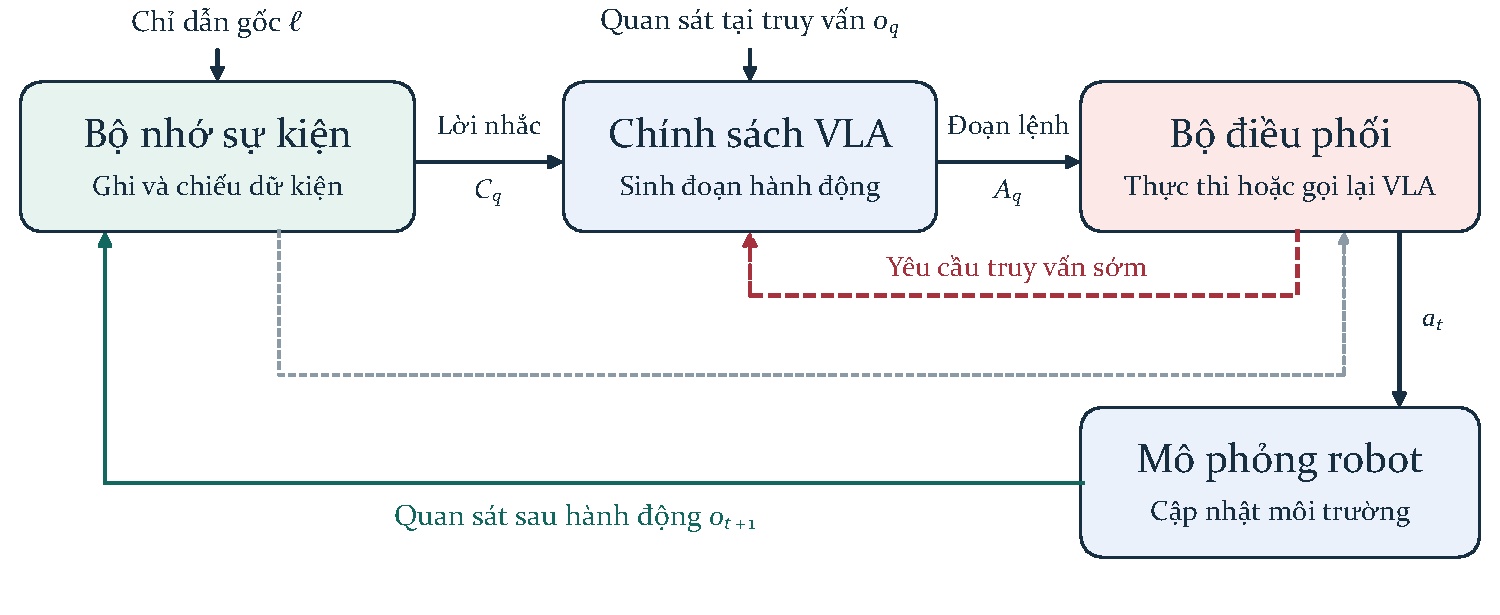
\includegraphics[width=\linewidth]{figures/vong-dieu-khien.pdf}
\caption{Vòng điều khiển VLA có bộ nhớ sự kiện}
\label{fig:architecture}
\end{figure}

%  Bộ đọc trích xuất dữ kiện có căn cứ để chiếu thành văn bản cho VLA sinh đoạn hành động. Bộ điều phối giám sát trực tiếp thay đổi trong bộ nhớ để kích hoạt quyền ngắt đoạn hành động
Trong đó $\ell$ là câu lệnh chỉ dẫn ngôn ngữ tổng thể của tác vụ, $M_t$ là trạng thái bộ nhớ sự kiện tại bước $t$, $C_q$ là ngữ cảnh ngôn ngữ được bộ đọc $R_B$ trích xuất và biểu diễn dưới ngân sách $B$ token tại thời điểm truy vấn $q$, và $A_q = (a_q, a_{q+1}, \ldots, a_{q+H-1})$ là đoạn hành động gồm $H$ bước liên tiếp do chính sách $\pi_{\theta,\phi}$ sinh ra từ quan sát hiện tại $o_q$ và ngữ cảnh $C_q$. Quy trình vận hành được điều phối khép kín: trước hết, bộ ghi cập nhật trạng thái bộ nhớ $M_t$ sau từng bước quan sát cảm biến $o_t$ và hành động vừa thực hiện $a_{t-1}$; thứ hai, tại mỗi bước truy vấn $q$, bộ đọc trích xuất các bằng chứng có căn cứ lịch sử, định dạng thành chuỗi văn bản ngắn $C_q$ không vượt quá $B$ token; thứ ba, chính sách VLA tiếp nhận cặp đầu vào $(o_q, C_q)$ để sinh đoạn hành động $A_q$; cuối cùng, bộ điều phối giám sát liên tục diễn biến của $M_t$ trong suốt quá trình robot thực thi đoạn hành động để quyết định có ngắt đoạn sớm hay không.

Tính an toàn của cơ chế này có thể được phân tích chặt chẽ qua lý thuyết xác suất sai số quyết định. Xét tình huống robot cần phân biệt hai trạng thái tiềm ẩn đồng xác suất (chẳng hạn vật nằm ở hộp X hoặc hộp Y) khi quan sát hiện tại hoàn toàn đồng nhất, sai số quyết định của chính sách phản xạ ngẫu nhiên là $1/2$. Giả sử bộ nhớ cung cấp câu trả lời với tỷ lệ bao phủ $c \in [0, 1]$ và tỷ lệ khẳng định sai là $\epsilon \in [0, 1]$. Áp dụng công thức xác suất toàn phần, kỳ vọng sai số quyết định của hệ thống được xác định bởi:

\begin{equation}
\mathbb E[\text{err}] = c\epsilon + \frac{1-c}{2} = \frac{1}{2} - c\left(\frac{1}{2} - \epsilon\right).
\label{eq:error-analysis}
\end{equation}

Phương trình~\eqref{eq:error-analysis} chỉ ra một kết quả lý thuyết quan trọng: kỳ vọng sai số toàn phần chỉ giảm so với chính sách phản xạ khi và chỉ khi tỷ lệ khẳng định sai thỏa mãn điều kiện $\epsilon < 1/2$. Ngược lại, nếu bộ nhớ đưa ra thông tin bị ảo giác với $\epsilon > 1/2$, việc tăng độ bao phủ $c$ sẽ làm tăng sai số toàn phần của hệ thống. Trong mô hình đơn giản này, việc giữ trạng thái \textit{chưa xác định} khi thiếu căn cứ quan sát tốt hơn việc suy đoán khi tỷ lệ khẳng định sai vượt $1/2$; mô hình chưa được kiểm chứng trên dữ liệu thực. Để tránh rò rỉ thông tin, kiến trúc thiết lập ranh giới phân tách độc lập hoàn toàn giữa nguồn thông tin của chính sách và nguồn đánh giá benchmark: bộ ghi và bộ đọc chỉ tiếp nhận dòng quan sát cảm biến được phép ($o_t$) mà không có quyền truy cập trạng thái môi trường đặc quyền, trong khi nhãn chân lý chỉ được sử dụng ở tầng đánh giá độc lập ngoại tuyến.

\section{Phương pháp bộ nhớ có bằng chứng}

\subsection{Cấu trúc bản ghi và tổ chức trạng thái}

Nhằm khắc phục triệt để hiện tượng mất dấu lịch sử và ảo giác thông tin, đơn vị lưu trữ cơ sở của bộ nhớ được thiết kế dưới dạng bản ghi sự kiện có cấu trúc tường minh:

\begin{equation}
f = (k, v, \sigma, \tau, \nu, I, \mathcal P).
\label{eq:record-tuple}
\end{equation}

Ý nghĩa toán học và chức năng của từng trường trong bộ bảy giá trị được định nghĩa như sau: trường khóa vị từ $k$ xác định tên quan hệ và vai trò định danh của các thực thể tham gia; trường giá trị $v$ lưu giữ giá trị chân lý, nhãn danh tính hoặc biến đếm tích lũy; trường trạng thái nhận thức $\sigma$ nhận giá trị trong tập gồm \textit{candidate} (ứng viên), \textit{confirmed} (xác nhận), \textit{unknown} (chưa rõ), \textit{conflicted} (mâu thuẫn), hoặc \textit{aborted} (hủy bỏ); trường $\tau$ ghi nhận thời điểm biến cố vật lý được ước lượng bắt đầu diễn ra trong môi trường thực; trường $\nu$ lưu giữ thời điểm xác nhận nhận thức ($\nu \ge \tau$), tức bước thời gian đầu tiên mà hệ thống tích lũy đủ chuỗi quan sát cảm biến phù hợp để chính thức xác nhận biến cố; trường khoảng thời gian hiệu lực $I = [t_{\mathrm{start}}, t_{\mathrm{end}}]$ xác định biên thời gian có giá trị của bản ghi (với sự kiện lịch sử thì $t_{\mathrm{end}} = \infty$, còn quan hệ hiện hành thì $t_{\mathrm{end}}$ kết thúc ngay khi có bằng chứng phủ định); và trường $\mathcal P$ lưu giữ tập chỉ mục nguồn gốc và căn cứ kiểm chứng gồm định danh khung ảnh cảm biến và tọa độ không gian để phục vụ truy vết nguyên nhân.

Để làm sáng tỏ ý nghĩa của cấu trúc trên, xét một bản ghi cụ thể ghi nhận biến cố robot đã hoàn thành việc đưa đồ vật A vào hộp X:

\begin{equation}
f_{\mathrm{ex}} = \Big(\underbrace{\text{In}(\text{obj}_A, \text{box}_X)}_{k},\ \underbrace{\text{true}}_{v},\ \underbrace{\text{confirmed}}_{\sigma},\ \underbrace{10}_{\tau},\ \underbrace{12}_{\nu},\ \underbrace{[10, \infty)}_{I},\ \underbrace{\mathcal P_{10:12}}_{\mathcal P}\Big).
\label{eq:record-example}
\end{equation}

Trong bản ghi mẫu này, tại bước thời gian vật lý $\tau = 10$, đồ vật A bắt đầu được đặt ổn định vào hộp X và tay kẹp robot mở ra. Tuy nhiên, để loại trừ rung lắc cảm biến, hệ thống yêu cầu điều kiện được thỏa mãn liên tục qua $p = 3$ quan sát liên tiếp, tức các bước 10, 11 và 12. Đến bước $\nu = 12$, khi vị từ hình học và trạng thái nhả kẹp được thỏa mãn liên tục, trạng thái nhận thức $\sigma$ chính thức được chuyển từ \textit{candidate} sang \textit{confirmed}. Khoảng hiệu lực $I = [10, \infty)$ phản ánh tính chất của một sự kiện lịch sử đã hoàn tất trong quá khứ (chân lý của biến cố này được bảo toàn vĩnh viễn trong tương lai của lượt thực thi), và tập căn cứ $\mathcal P_{10:12} = \{(\text{rgb}_t, \mathbf b_t^{\mathrm{obj}}, \text{grip}_t)\}_{t=10}^{12}$ lưu giữ đầy đủ mã định danh khung ảnh, tọa độ hộp bao và độ mở tay kẹp từ bước 10 đến 12 để phục vụ việc kiểm chứng và truy vết nguyên nhân khi cần thiết.

Việc phân tách ranh giới giữa thời điểm vật lý $\tau$ và thời điểm xác nhận nhận thức $\nu$ là một đóng góp thiết kế quan trọng. Một sự kiện thao tác có thể bắt đầu diễn ra ở bước $\tau = 10$, nhưng cảm biến cần quan sát thêm hai bước tiếp theo để xác nhận sự ổn định vật lý, dẫn tới thời điểm đủ căn cứ là $\nu = 12$. Trong trường hợp này, thông tin sự kiện tuyệt đối không được phép xuất hiện trong ngữ cảnh suy luận tại bước 10 hay 11, ngăn chặn triệt để hiện tượng rò rỉ thông tin tương lai trong cả pha huấn luyện lẫn pha suy luận.

Toàn bộ tri thức tích lũy của robot đến bước thời gian $t$ được tổ chức thành trạng thái bộ nhớ bốn thành phần:

\begin{equation}
M_t = (\mathcal O_t, \mathcal R_t, \mathcal E_t, \mathcal P_t).
\label{eq:memory-state}
\end{equation}

Trong đó $\mathcal O_t$ là tập hợp các thực thể và giả thuyết định danh đang được hệ thống duy trì, $\mathcal R_t$ là tập hợp các quan hệ trạng thái đang còn hiệu lực tại bước $t$, $\mathcal E_t$ là tập hợp các sự kiện lịch sử đã được xác nhận hoàn tất trong quá khứ, và $\mathcal P_t$ là chỉ mục tham chiếu bằng chứng và nguồn gốc dữ liệu.

\begin{figure}[htbp]
\centering
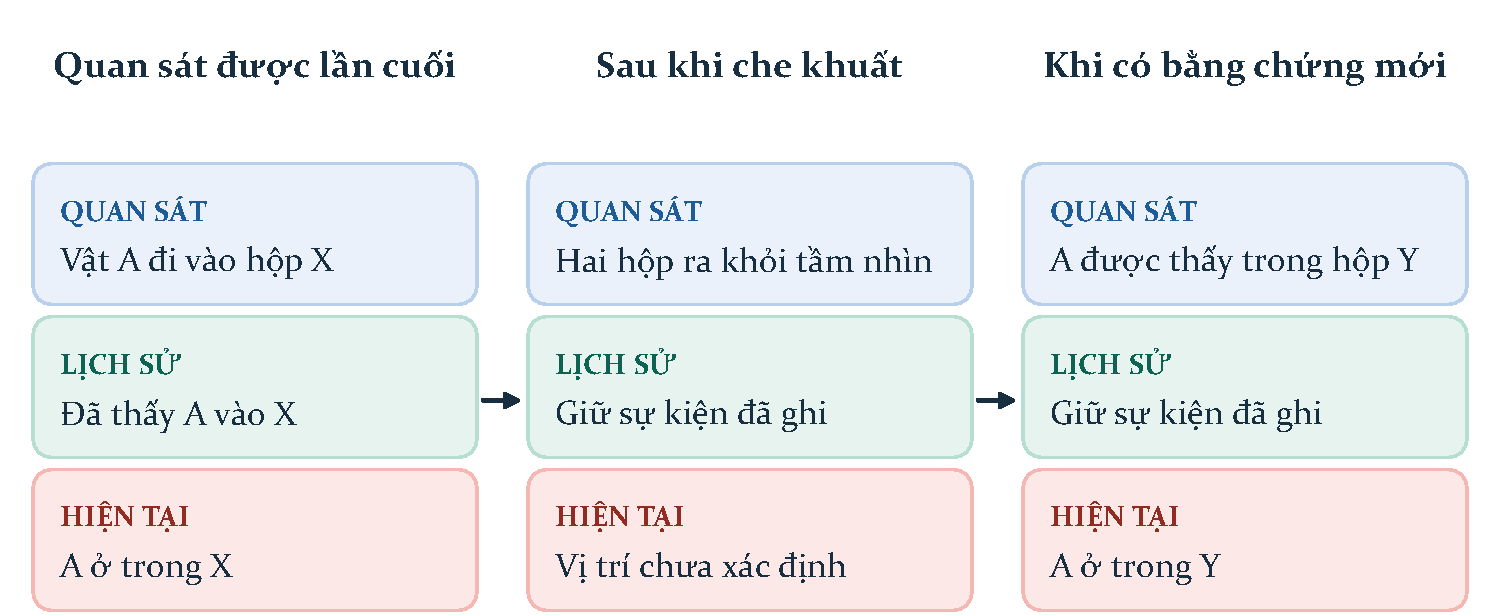
\includegraphics[width=.95\textwidth]{figures/su-kien-che-khuat.pdf}
\caption{Sự kiện lịch sử và quan hệ hiện tại khi vật bị che khuất}
\label{fig:memory-evidence-states}
\end{figure}

Như được minh họa ở Hình~\ref{fig:memory-evidence-states}, sự phân định giữa $\mathcal R_t$ và $\mathcal E_t$ phản ánh sự khác biệt căn bản về mặt nhận thức học. Sự kiện lịch sử ($\mathcal E_t$) mô tả một biến cố đã xảy ra trong quá khứ dựa trên quan sát thực tế tại thời điểm đó, có tính chân lý bất biến theo thời gian và không bị hủy bỏ bởi các diễn biến che khuất sau đó. Ngược lại, quan hệ hiện hành ($\mathcal R_t$) mô tả trạng thái không gian tại thời điểm hiện tại và chỉ có hiệu lực chừng nào các điều kiện bảo toàn vật lý được duy trì; nếu vật thể bị che khuất hoặc di chuyển khỏi tầm quan sát tin cậy, quan hệ trong $\mathcal R_t$ buộc phải chuyển trạng thái sang \textit{chưa xác định}. Cấu trúc này cho phép bộ nhớ đáp ứng linh hoạt cả ba dạng truy vấn trọng yếu: truy vấn không gian hiện tại từ $\mathcal R_t$, truy vấn ngữ cảnh quá khứ từ $\mathcal E_t$, và truy vấn tiến độ thao tác thông qua phép tổng hợp và đếm trên tập sự kiện $\mathcal E_t$.

\subsection{Nguyên lý trích xuất và kiểm định bằng chứng}

Để khung bộ nhớ có thể vận hành tổng quát trên nhiều tác vụ mà không bị phụ thuộc vào các ngưỡng tham số cục bộ, quá trình trích xuất và kiểm định bằng chứng được thiết kế dựa trên ba nguyên tắc cốt lõi: chuẩn hóa quan hệ hình học theo kích thước vật thể, bảo lưu danh tính thực thể khi bị che khuất, và khử nhiễu cảm biến thông qua cơ chế xác nhận trễ thời gian.

Trước hết, từ mỗi quan sát cảm biến $o_t$, hệ thống xác định vị trí và hộp bao của các thực thể liên quan. Nhằm loại bỏ hoàn toàn sự phụ thuộc vào góc đặt camera, cự ly quan sát và kích thước vật lý riêng của từng đồ vật, quan hệ không gian được đánh giá dựa trên độ dịch chuyển tương đối đã được chuẩn hóa theo kích thước của đối tượng mốc:

\begin{equation}
d_t = (\mathbf x_t^{\mathrm{obj}} - \mathbf x_t^{\mathrm{ref}}) - (\mathbf x_0^{\mathrm{obj}} - \mathbf x_0^{\mathrm{ref}}),\qquad
D_t = \left\| d_t \oslash \mathbf w_{\mathrm{ref}} \right\|_2.
\label{eq:scale-invariant-distance}
\end{equation}

Trong đó $\mathbf x_t^{\mathrm{obj}}$ và $\mathbf x_t^{\mathrm{ref}}$ lần lượt là tọa độ trung tâm của vật thể thao tác và đối tượng tham chiếu mốc tại bước $t$, $\mathbf w_{\mathrm{ref}}$ là kích thước hình học biểu kiến của đối tượng mốc, và $\oslash$ biểu thị phép chia theo từng thành phần tọa độ. Đại lượng vô hướng $D_t$ cung cấp một chỉ số đo khoảng cách tương đối không thứ nguyên, phản ánh mức độ thay đổi vị trí một cách nhất quán bất kể vật thể lớn hay nhỏ, đặt gần hay xa camera.

Thứ hai, nhằm duy trì tính nhất quán nhận thức trong suốt chuỗi thao tác, hệ thống cần bảo lưu chính xác danh tính của từng thực thể ngay cả khi xảy ra va chạm hay che khuất. Bằng cách liên kết các phát hiện thị giác tại bước $t$ với tập thực thể $\mathcal O_{t-1}$ dựa trên vị trí không gian kết hợp với đặc trưng diện mạo, hệ thống nhận biết liên tục đối tượng nào đang được thao tác. Khi một thực thể tạm thời bị che khuất bởi ngón kẹp robot hoặc di chuyển khỏi tầm nhìn của camera, trạng thái của nó được chuyển sang \textit{occluded} nhưng danh tính và lịch sử tương tác vẫn được duy trì trong bộ nhớ, thay vì bị xóa bỏ hoặc bị nhận diện nhầm thành một vật thể mới.

Thứ ba, do dữ liệu thị giác từ camera thường chịu ảnh hưởng bởi nhiễu hoặc sai số, hệ thống áp dụng cơ chế xác nhận trễ thời gian với độ dài cửa sổ $p$ quan sát. Một biến cố trạng thái không bao giờ được kích hoạt chỉ sau một quan sát riêng lẻ; thay vào đó, biến cố chỉ chính thức chuyển từ trạng thái ứng viên sang trạng thái xác nhận khi vị từ tương ứng duy trì giá trị thỏa mãn liên tục qua ít nhất $p$ bước quan sát kế tiếp nhau, trong đó $\phi_k$ là hàm vị từ ứng với khóa $k$:

\begin{equation}
\sigma_t = \text{confirmed} \iff \forall i \in [t - p + 1, t],\ \phi_k(o_i) = \text{true}.
\label{eq:temporal-hysteresis}
\end{equation}

Tiến trình thao tác tổng thể được quản lý bởi một máy trạng thái hữu hạn. Gọi $J_t$ là số chu kỳ thao tác đã bắt đầu, $\hat z_t$ là số chu kỳ đã hoàn thành hợp lệ được bộ nhớ xác nhận, $X_t$ là số chu kỳ bị hủy bỏ do vi phạm điều kiện an toàn, và $\chi_t$ là biến trạng thái chỉ thị chu kỳ hiện tại đang diễn ra ($\chi_t = 1$) hay hệ thống đang ở trạng thái nghỉ ($\chi_t = 0$). Tiến trình của hệ thống luôn thỏa mãn FSM invariant:

\begin{equation}
J_t - \hat z_t - X_t = \chi_t,\qquad \chi_t \in \{0, 1\}.
\label{eq:fsm-invariant}
\end{equation}

Bất biến~\eqref{eq:fsm-invariant} cho biết tại mọi bước, tổng số chu kỳ đã hoàn thành, đã hủy và đang diễn ra luôn bằng số chu kỳ đã bắt đầu, nên máy trạng thái không thể bỏ qua một chuyển tiếp. Bất biến này được kiểm tra bằng quy nạp theo từng chuyển tiếp của FSM: mỗi chuyển tiếp hợp lệ chỉ làm thay đổi đúng một trong các đại lượng $J_t$, $\hat z_t$, $X_t$ và giữ $\chi_t \in \{0,1\}$. Đặc tính nhân quả chặt chẽ của toàn bộ quy trình trích xuất và chiếu ngữ cảnh được khẳng định qua mệnh đề sau.

\textbf{Mệnh đề 1: Tính không nhìn trước của ngữ cảnh chiếu.} Giả sử hai quỹ đạo tương tác có cùng tiền tố quan sát và hành động đến bước truy vấn $q$, tức $h_q = h'_q$. Khi đó trạng thái bộ nhớ và ngữ cảnh chiếu tại bước $q$ là hoàn toàn đồng nhất:

\begin{equation}
h_q = h'_q \implies M_q = M'_q \implies R_B(\ell, M_q) = R_B(\ell, M'_q).
\label{eq:non-anticipatory}
\end{equation}

\textbf{Chứng minh.} Tại bước khởi đầu $t=0$, hai quỹ đạo có cùng cấu hình và quan sát ban đầu $o_0 = o'_0$, do đó $M_0 = M'_0$. Giả sử quy nạp rằng $M_{t-1} = M'_{t-1}$ với mọi $t \le q$. Vì hai tiền tố giống hệt nhau $h_q = h'_q$, ta có $o_t = o'_t$ và $a_{t-1} = a'_{t-1}$. Do quy tắc cập nhật $U$ là một hàm xác định, ta suy ra $M_t = U(M_{t-1}, o_t, a_{t-1}) = U(M'_{t-1}, o'_t, a'_{t-1}) = M'_t$. Áp dụng quy nạp đến bước $q$, ta thu được $M_q = M'_q$. Cuối cùng, vì phép chiếu $R_B$ chỉ đọc các bản ghi trong $M_q$ có $\nu \le q$, hai trạng thái bộ nhớ giống nhau sẽ sinh ra cùng một tập sự kiện được chọn $S_q = S'_q$ và cùng một chuỗi văn bản $C_q = C'_q$. $\blacksquare$

\begin{figure}[htbp]
\centering
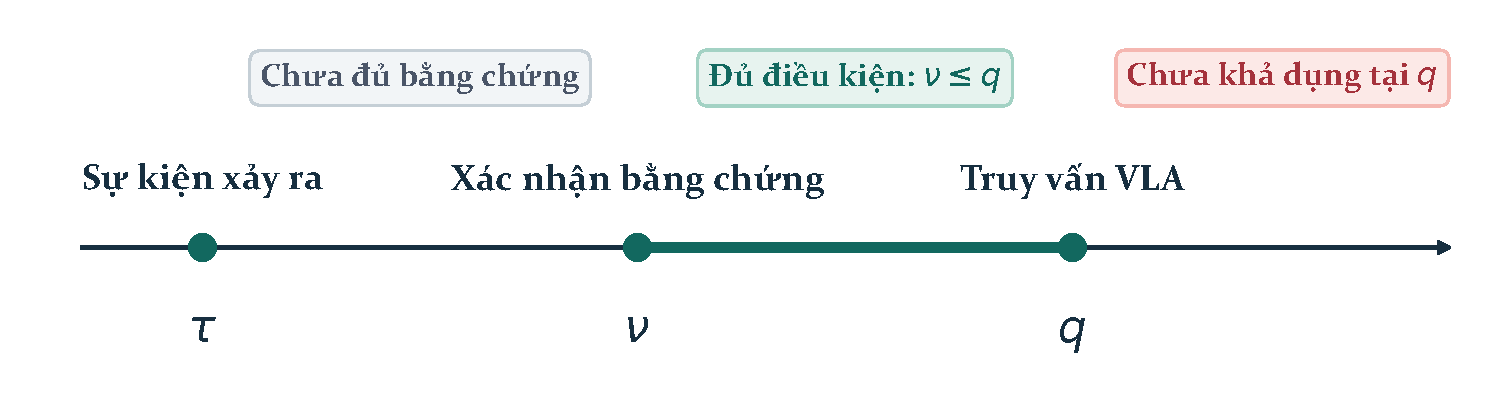
\includegraphics[width=.93\textwidth]{figures/truc-bang-chung.pdf}
\caption{Thời điểm xảy ra, xác nhận và truy vấn sự kiện}
\label{fig:memory_timeline}
\end{figure}

Mệnh đề 1 bảo đảm rằng ngữ cảnh được bộ nhớ cấp cho VLA hoàn toàn là hệ quả nhân quả của các quan sát quá khứ, loại bỏ khả năng mô hình học vẹt hoặc dựa trên rò rỉ tương lai như minh họa ở Hình~\ref{fig:memory_timeline}.

\subsection{Các trường hợp cụ thể với tác vụ}

Để áp dụng khung bộ nhớ trên các lớp tác vụ khác nhau, hệ thống định nghĩa một giao thức bộ nhớ theo tác vụ $T_{\mathrm{spec}} = (\Phi, \Delta, \mathcal{F})$, trong đó $\Phi$ là tập các hàm vị từ, $\Delta$ là tập các quy tắc chuyển trạng thái FSM, và $\mathcal{F}$ là định dạng chuỗi chiếu văn bản. LIBERO-Mem \cite{liberomem2025} chia mười tác vụ thành bốn nhóm năng lực bộ nhớ: OM (Object Motion, nhớ lịch sử chuyển động và trạng thái tương tác của từng vật thể), OS (Object Sequence, nhớ số lần và thứ tự tương tác), OR (Object Relations, nhớ quan hệ và vị trí giữa nhiều vật thể) và OO (Object Occlusion, nhớ danh tính và vị trí vật thể khi bị che khuất). Một tác vụ có thể thuộc nhiều nhóm. Bảng~\ref{tab:memory-task-families} tổng hợp nhóm năng lực và các primitive lịch sử cần thiết cho mười tác vụ này.

\begingroup\small\setlength{\tabcolsep}{4pt}\renewcommand{\arraystretch}{1.12}
\begin{longtable}{>{\raggedright\arraybackslash}p{.12\textwidth}|>{\raggedright\arraybackslash}p{.28\textwidth}|>{\raggedright\arraybackslash}p{.52\textwidth}}
\caption{Dạng thông tin lịch sử theo tác vụ LIBERO-Mem}\label{tab:memory-task-families}\\
\toprule
\textbf{Tác vụ} & \textbf{Lớp bài toán lịch sử} & \textbf{Primitive trừu tượng cần biểu diễn} \\
\midrule\endfirsthead
\toprule
\textbf{Tác vụ} & \textbf{Lớp bài toán lịch sử} & \textbf{Primitive trừu tượng cần biểu diễn} \\
\midrule\endhead
\bottomrule\endfoot
T1 & Đơn chu kỳ (OM) & Một chu kỳ nhấc và hoàn nguyên vật thể về mốc ban đầu \\
T2 & Tương tác trạng thái (OM) & Trạng thái tương tác tiếp xúc giữa hai vật thể \\
T3 & Đa chu kỳ ngắn (OM, OS) & Đếm và phân biệt tiến độ ba chu kỳ thao tác lặp lại \\
T4 & Đa chu kỳ tương tác (OM, OS) & Đếm số lần tương tác có chủ đích với vật thể \\
T5 & Đa chu kỳ trung bình (OM, OS) & Duy trì bộ đếm sự kiện qua năm chu kỳ liên tiếp \\
T6 & Đa chu kỳ dài (OM, OS) & Duy trì bộ đếm sự kiện qua bảy chu kỳ liên tiếp \\
T7 & Hoán đổi không gian (OM, OR) & Theo dõi quan hệ vị trí của hai vật thể qua ba mốc hoán đổi \\
T8 & Xoay vòng vị trí (OM, OR) & Theo dõi danh tính và vị trí của ba vật thể qua chuỗi xoay vòng \\
T9 & Vật chứa di chuyển (OM, OO) & Duy trì quan hệ chứa khi đối tượng chứa bị di chuyển \\
T10 & Phân biệt vật chứa (OM, OO) & Phân biệt vật chứa có chứa đồ vật với vật chứa rỗng sau che khuất \\
\end{longtable}
\endgroup

Khung giao thức này khẳng định tính tổng quát của phương pháp: các dạng bài toán từ đếm chu kỳ thao tác (OM/OS), theo dõi hoán đổi vị trí (OR) đến duy trì quan hệ vật chứa khi che khuất (OO) đều có thể được chuẩn hóa dưới dạng các bản ghi sự kiện có bằng chứng $f = (k, v, \sigma, \tau, \nu, I, \mathcal P)$.

Để chứng minh tính khả thi, nghiên cứu xây dựng một trường hợp cụ thể hóa điển hình: Bộ theo dõi chu kỳ thao tác lặp lại đối với vật thể trên mặt bàn bằng camera RGB. Trong trường hợp hiện thực này, vật thể thao tác và mốc tham chiếu được trích xuất tọa độ thông qua các hộp bao thị giác 2D từ camera ngoài và camera cổ tay. Gọi $\mathbf b_t$ và $\mathbf q_t$ lần lượt là tâm mép dưới của hộp bao vật thể và mốc vị trí tại bước $t$, $(w_b, h_b)$ là kích thước hộp bao vật thể tại thời điểm xác lập mốc ban đầu. Các đại lượng hình học tương đối được tính toán theo Phương trình~\eqref{eq:scale-invariant-distance}:

\begin{equation}
d_t = (\mathbf b_t - \mathbf q_t) - (\mathbf b_0 - \mathbf q_0),\qquad
D_t = \left\| d_t \oslash (w_b, h_b) \right\|_2,\qquad
L_t = -d_{t,y} / h_b.
\label{eq:case-study-geometry}
\end{equation}

Trong đó $D_t$ đo độ lệch mặt bằng đã chuẩn hóa, $L_t$ đo độ dịch chuyển nâng lên theo phương thẳng đứng của ảnh. Bảng~\ref{tab:case-study-thresholds} trình bày chi tiết các tiêu chí định lượng được cấu hình cho trường hợp cụ thể hóa này.

\begingroup\small\setlength{\tabcolsep}{4pt}\renewcommand{\arraystretch}{1.15}
\begin{longtable}{>{\raggedright\arraybackslash}p{\dimexpr 0.25\textwidth-2\tabcolsep\relax}|>{\raggedright\arraybackslash}p{\dimexpr 0.35\textwidth-2\tabcolsep\relax}|>{\raggedright\arraybackslash}p{\dimexpr 0.4\textwidth-2\tabcolsep\relax}}
\caption{Ngưỡng theo dõi chu kỳ thao tác}\label{tab:case-study-thresholds}\\
\toprule
\textbf{Đại lượng kiểm tra} & \textbf{Tiêu chí định lượng} & \textbf{Vai trò nhận thức trong quy trình} \\
\midrule\endfirsthead
\toprule
\textbf{Đại lượng kiểm tra} & \textbf{Tiêu chí định lượng} & \textbf{Vai trò nhận thức trong quy trình} \\
\midrule\endhead
\bottomrule\endfoot
Điểm tin cậy phát hiện & $s_{\mathrm{det}} \ge 0{,}15$ & Lọc các đề xuất hộp bao đạt ngưỡng chất lượng \\
Ứng viên rời mốc & $L_t \ge 0{,}40$ và ra khỏi vùng lân cận mốc & Xác định thời điểm vật thể bắt đầu được nâng lên \\
Ứng viên quay về mốc & $D_t \le 0{,}30$, tỷ lệ rộng $[0{,}6; 1{,}5]$, cao $[0{,}3; 1{,}5]$ & Nhận diện vật thể đã quay về vùng không gian của mốc \\
Trạng thái ổn định & Độ dịch tâm mép dưới chuẩn hóa $\le 0{,}15$ & Xác nhận vật thể đã ổn định vị trí, không còn chuyển động \\
Tay kẹp mở hoàn toàn & Tổng độ mở hai khớp ngón kẹp $\ge 0{,}055$ m & Căn cứ vật lý bổ trợ xác nhận robot đã nhả vật thể \\
Xác nhận trễ thời gian & Duy trì phù hợp qua $p = 3$ bước liên tiếp & Cửa sổ xác nhận chống nhiễu đơn khung hình \\
Liên kết mốc tham chiếu & Khoảng cách 2D với mốc $\le 0{,}20$ và IoU $\ge 0{,}10$ & Kiểm tra vật thể đã hoàn nguyên đúng tọa độ ban đầu \\
\end{longtable}
\endgroup

Quy tắc sinh sự kiện hoàn thành chu kỳ được cụ thể hóa bằng điều kiện logic kết hợp đa phương thức:

\begin{equation}
\operatorname{Event}_{\mathrm{cycle\_complete}}(t) \iff
\left(
\begin{aligned}
&\text{State}_{t-1} = \text{lifted} \;\land\; D_t \le 0{,}30 \;\land\; L_t \le 0{,}15 \\
&\land\; \operatorname{Stable}(t, p) \;\land\; \operatorname{GripperOpen}(t)
\end{aligned}
\right).
\label{eq:event-rule-instantiation}
\end{equation}

Khi điều kiện Phương trình~\eqref{eq:event-rule-instantiation} thỏa mãn, bộ ghi ghi nhận một sự kiện hoàn thành chu kỳ mới vào $\mathcal E_t$, cập nhật bộ đếm tiến độ $\hat z_t \leftarrow \hat z_{t-1} + 1$, chuyển trạng thái FSM về $\text{idle}$, và giải phóng biến theo vết để sẵn sàng cho chu kỳ tiếp theo nếu tác vụ yêu cầu.

\section{Quy trình huấn luyện thích ứng}
\label{sec:adaptation}

Để chính sách VLA có khả năng tiếp nhận và khai thác hiệu quả tín hiệu bộ nhớ mà không phá vỡ khả năng thao tác cơ sở đã học trong giai đoạn tiền huấn luyện, khóa luận xây dựng một quy trình huấn luyện thích ứng có kiểm soát. Quy trình gồm ba bước dùng chung cho mọi mô hình nền; chỉ tập tham số được cập nhật ở bước thứ ba phụ thuộc vào kiến trúc cụ thể.

Trước hết, từ tập dữ liệu quỹ đạo mẫu chuyên gia, hệ thống áp dụng cơ chế chạy lại bộ ghi ngoại tuyến để sinh các mẫu huấn luyện theo đúng tiền tố nhân quả. Tại mỗi điểm truy vấn mẫu $q$, bộ ghi chỉ xử lý chuỗi quan sát quá khứ $o_{0:q}$ để tạo ra trạng thái bộ nhớ $M_q$ và chuỗi văn bản tương ứng $C_q = R_B(\ell, M_q)$. Mẫu huấn luyện được cấu trúc thành bộ ba $(o_q, C_q, A_q^{\mathrm{demo}})$, trong đó $A_q^{\mathrm{demo}}$ là đoạn $H$ hành động liên tiếp của chuyên gia bắt đầu từ bước $q$. Việc tạo mẫu ngoại tuyến nghiêm ngặt này loại bỏ hoàn toàn nguy cơ rò rỉ thông tin tương lai vào ngữ cảnh huấn luyện.

Thứ hai, để giải quyết hiện tượng quên thảm khốc khi tinh chỉnh trên dữ liệu mới, nghiên cứu áp dụng chiến lược lấy mẫu cân bằng hai miền dữ liệu. Tập dữ liệu huấn luyện được hòa trộn đồng đều theo tỷ lệ $1:1$ giữa tập dữ liệu có bộ nhớ $\mathcal D_{\mathrm{mem}}$ (gồm các quỹ đạo thao tác đa chu kỳ kèm ngữ cảnh tiến độ) và tập dữ liệu thao tác cơ sở $\mathcal D_{\mathrm{base}}$ (các tác vụ đơn lẻ không kèm bộ nhớ). Mục tiêu tối ưu hóa được xác định bởi hàm mất mát Flow Matching kết hợp trên cả hai miền dữ liệu:

\begin{equation}
\min_\phi \frac{1}{2} \mathbb E_{(o, C, A) \sim \mathcal D_{\mathrm{base}}} \mathcal L_{\mathrm{flow}}(\theta, \phi; o, C, A) + \frac{1}{2} \mathbb E_{(o, C, A) \sim \mathcal D_{\mathrm{mem}}} \mathcal L_{\mathrm{flow}}(\theta, \phi; o, C, A).
\label{eq:training-loss}
\end{equation}

Trong đó $\theta$ biểu thị các trọng số được đóng băng của mô hình nền, $\phi$ là tập tham số thích ứng được tối ưu, và $\mathcal L_{\mathrm{flow}}$ là hàm mất mát hồi quy trường vận tốc dòng chảy dòng hành động.

Thứ ba, tập tham số thích ứng $\phi$ được chọn theo kiến trúc của từng mô hình nền, trong khi dữ liệu, ngân sách cập nhật và cách tạo lời nhắc giữ nguyên giữa F0 và F1. Với SmolVLA, nghiên cứu thích ứng action expert bằng LoRA như Hình~\ref{fig:smolvla-lora}: các phép chiếu truy vấn $W_q$ và giá trị $W_v$ trong các tầng attention của action expert được bổ sung nhánh hạng thấp $W + \frac{\alpha}{r} B_{\mathrm{L}} A_{\mathrm{L}}$, với hạng $r = 16$ và hệ số tỉ lệ $\alpha = 32$. Quá trình huấn luyện cập nhật 645.120 tham số LoRA và giữ cố định các trọng số gốc của action expert, bộ mã hóa ảnh SigLIP, mô hình ngôn ngữ SmolLM2 và các mô-đun còn lại. Với X-VLA, tập $\phi$ gồm các ma trận LoRA và một số mô-đun được huấn luyện đầy đủ, tổng cộng khoảng 11,87 triệu tham số; cấu hình chi tiết được nêu ở Mục~\ref{sec:xvla-setup}.

\begin{figure}[htbp]
\centering
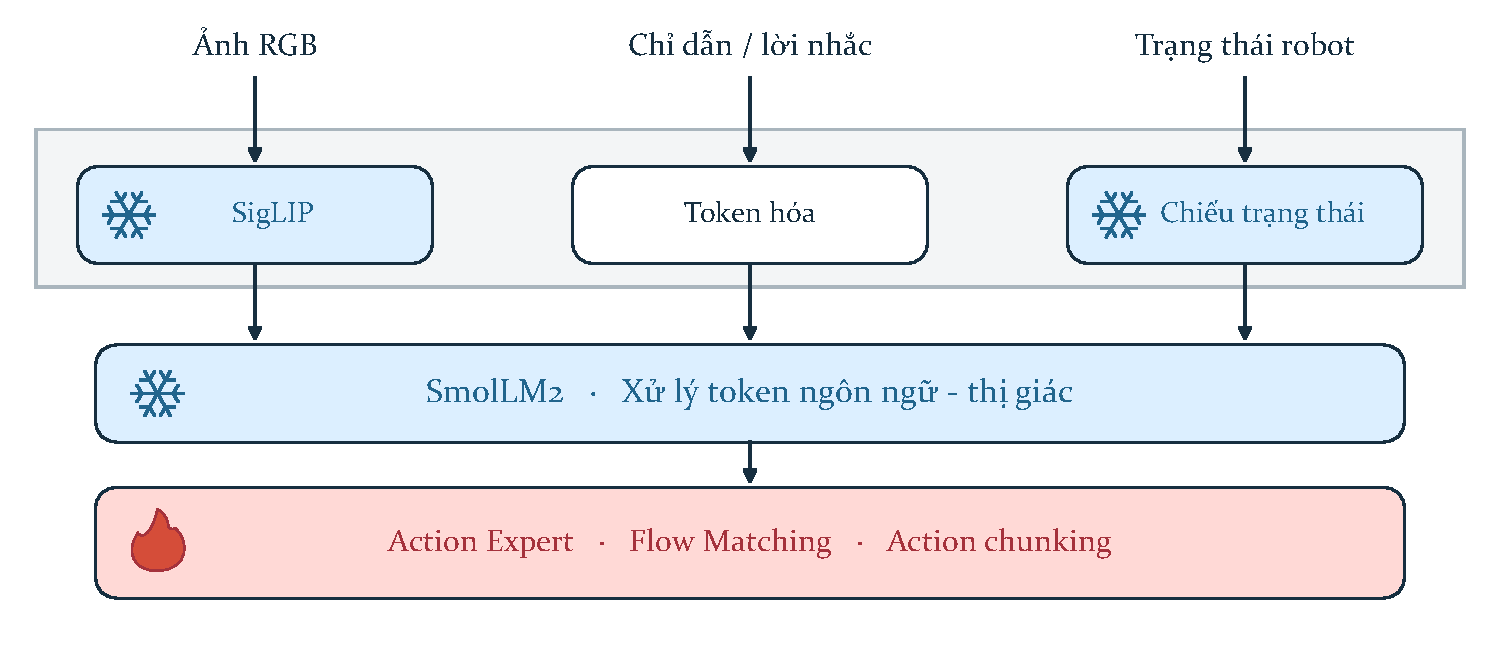
\includegraphics[width=.96\linewidth]{figures/smolvla-lora.pdf}
\caption{Phần đóng băng và phần tinh chỉnh LoRA trong SmolVLA}
\label{fig:smolvla-lora}
\end{figure}

\section{Suy luận và điều phối hành động theo thời gian thực}

Trong pha triển khai vận hành trực tuyến, chính sách VLA tích hợp bộ nhớ phải đáp ứng hai yêu cầu khắt khe: tuân thủ nghiêm ngặt ngân sách độ dài token đầu vào để duy trì tần số suy luận cao, và điều phối nhịp thực thi hành động linh hoạt nhằm phản ứng kịp thời với các biến cố môi trường.

Về mặt biểu diễn ngữ cảnh, bộ đọc áp dụng cơ chế chiếu nén có kiểm soát ngân sách: từ trạng thái bộ nhớ hiện tại $M_q$, bộ đọc lọc các bản ghi có căn cứ nhân quả $\nu \le q$, còn hiệu lực thời gian và có liên quan trực tiếp đến chỉ dẫn tác vụ $\ell$ để định dạng thành chuỗi văn bản tự nhiên $C_q$:

\begin{equation}
S_q = \operatorname{Select}(\ell, M_q, B),\qquad C_q = \operatorname{Render}(\ell, S_q),\qquad |\operatorname{Enc}(C_q)| \le B.
\label{eq:context-projection}
\end{equation}

Ngân sách độ dài được ấn định nghiêm ngặt ở mức $B = 48$ token cho toàn bộ văn bản đầu vào. Quy định này bảo đảm số lượng token đưa vào mô hình VLA luôn là một hằng số cố định, không phụ thuộc vào độ dài thời gian của quỹ đạo hay số lượng sự kiện đã tích lũy trong quá khứ, nên chi phí văn bản không tăng theo độ dài lượt chạy.

Về mặt điều phối thực thi, trong mô hình Action Chunking truyền thống, robot thực thi liên tục toàn bộ $H$ hành động trong đoạn theo chu kỳ cố định $s$ bước mới tái truy vấn VLA một lần. Nhược điểm lớn của cơ chế cố định này là độ trễ phản xạ cao: nếu một biến cố then chốt xảy ra ngay ở đầu đoạn hành động (chẳng hạn vật đã rơi vào đúng đích ở bước thứ 2 của đoạn $s = 10$), robot vẫn phải thực hiện 8 hành động còn lại trước khi nhận được trạng thái mới, gây lãng phí hoặc thao tác thừa. Để khắc phục, hệ thống triển khai cơ chế ngắt đoạn hành động động dựa trên bằng chứng: bộ điều phối giám sát liên tục diễn biến của $M_t$ sau mỗi bước thực thi hành động $t$. Khi phát hiện một thay đổi bằng chứng ngữ nghĩa có liên quan được duy trì ổn định qua $p$ quan sát liên tiếp và robot đã hoàn thành tối thiểu $k_{\min}$ hành động từ lần truy vấn trước, thời điểm truy vấn tiếp theo $q'$ được kích hoạt sớm. Gọi $e_t \in \{0,1\}$ là chỉ báo bằng chứng mới đã được xác nhận tại bước $t$, ta có:

\begin{equation}
q' = \min\!\left(q + s,\ \inf\{t > q : t - q \ge k_{\min},\ e_t = 1\}\right).
\label{eq:dynamic-preemption}
\end{equation}

Như minh họa tại Hình~\ref{fig:evidence-requery}, khi điều kiện ngắt được thỏa mãn tại $q'$, bộ điều phối lập tức hủy bỏ các hành động chưa thực thi trong đoạn cũ, lấy quan sát mới $o_{q'}$, chiếu ngữ cảnh cập nhật $C_{q'}$ và kích hoạt VLA sinh đoạn hành động mới.

\begin{figure}[htbp]
\centering
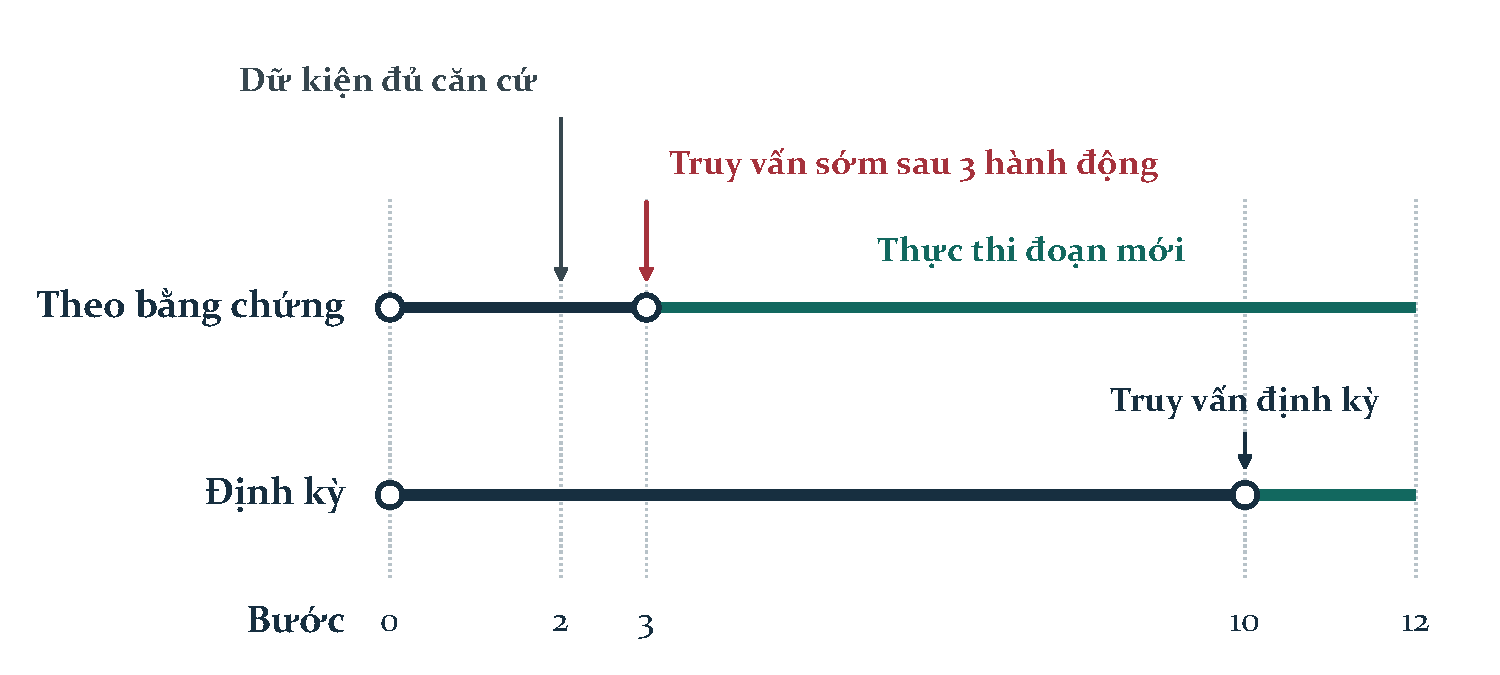
\includegraphics[width=.94\textwidth]{figures/truy-van-som.pdf}
\caption{Truy vấn sớm khi có bằng chứng mới}
\label{fig:evidence-requery}
\end{figure}

Hiệu quả phản ứng của cơ chế ngắt động có thể được chứng minh qua định lý chặn trên thời gian trễ.

\textbf{Mệnh đề 2: Chặn trên của độ trễ với biến cố mới.} Giả sử robot đang thực thi đoạn hành động được sinh tại bước $q$. Một biến cố trạng thái mới xuất hiện trong môi trường tại thời điểm $r$ (với $q < r \le q + s$) và duy trì liên tục. Nếu không có biến cố nào khác kích hoạt trước đó, thời điểm tái truy vấn chính sách $q'$ thỏa mãn:

\begin{equation}
q' = \min(q + s,\ \max(q + k_{\min},\ r + p - 1)).
\label{eq:latency-formula}
\end{equation}

Hệ quả là số bước hành động robot tiếp tục sử dụng đoạn điều khiển cũ sau khi biến cố xuất hiện, trong đó $r$ là thời điểm bộ ghi bắt đầu quan sát thấy biến cố, bằng:

\begin{equation}
q' - r = \min\!\big(q + s - r,\ \max(q + k_{\min} - r,\ p - 1)\big) \le q + s - r.
\label{eq:latency-bound}
\end{equation}

\textbf{Chứng minh.} Biến cố xuất hiện tại bước $r$. Do quy tắc lọc trễ thời gian đòi hỏi $p$ quan sát liên tiếp để xác nhận, thời điểm sớm nhất biến cố được xác nhận là $t_{\mathrm{confirm}} = r + p - 1$, tại đó $e_t = 1$. Đồng thời, cơ chế điều phối đòi hỏi robot phải thực thi tối thiểu $k_{\min}$ hành động từ lần truy vấn trước, tức $t \ge q + k_{\min}$. Do đó, bước thời gian sớm nhất thỏa mãn đồng thời cả hai điều kiện là $t = \max(q + k_{\min}, r + p - 1)$. Mặt khác, lịch truy vấn định kỳ chặn trên thời điểm gọi tiếp theo tại $q + s$. Kết hợp hai điều kiện, ta thu được $q' = \min(q + s, \max(q + k_{\min}, r + p - 1))$. Trừ $r$ ở hai vế của công thức trên ta được độ trễ nêu ở phương trình sau. Độ trễ thực tế của bộ ghi, được đo ở Chương 4 là từ 4 đến 30 bước đối với bộ ghi thị giác, cộng thêm vào $r$. $\blacksquare$

Công thức Phương trình~\eqref{eq:latency-formula} cho thấy rõ sự linh hoạt của cơ chế: khi biến cố được xác nhận sớm ($r + p - 1 < q + s$), hệ thống truy vấn lại ngay khi đã thực thi tối thiểu $k_{\min}$ hành động, nên độ trễ phản ứng nhỏ hơn so với việc thực thi hết chu kỳ $s$.

Bộ điều phối có thể mở rộng sang suy luận bất đồng bộ, trong đó luồng điều khiển và luồng truy vấn chạy song song và mỗi đề xuất được kiểm tra lại với phiên bản bộ nhớ khi hoàn tất. Tuy nhiên, hướng này không phải mục tiêu chính để cài đặt và đánh giá trong khóa luận này.

\textbf{Cơ chế dừng thực thi dựa trên bằng chứng bộ nhớ.}
\label{sec:method-memory-halt}

Bộ điều phối ở phần trước chỉ giải quyết bài toán thời điểm kích hoạt truy vấn lại chính sách, và mặc định giả định rằng mô hình VLA có thể tự nhận biết thời điểm kết thúc nhiệm vụ. Tuy nhiên, giả định này thường không thỏa mãn trong thực tế đối với các chính sách học từ quỹ đạo minh họa mẫu. Do dữ liệu minh họa thường kết thúc ngay khi mốc tác vụ cuối cùng đạt điều kiện, chính sách hiếm khi được quan sát trạng thái đứng yên sau khi hoàn thành, dẫn đến khuynh hướng tiếp tục thực thi thao tác thừa gây mất kết quả đã đạt, gọi là hiện tượng overshoot. Thông tin mà chính sách còn thiếu chính là tiến độ tích lũy theo thời gian, đúng với đại lượng mà bộ nhớ sự kiện liên tục cập nhật. Do đó, không gian quyết định của bộ điều phối được mở rộng thành ba trạng thái gồm tiếp tục thực thi, truy vấn lại sớm hoặc dừng hẳn thao tác, mà không làm xáo trộn không gian trọng số hay ngữ cảnh chiếu $C_q$.

Về mặt hình thức, gọi $z_t$ là tiến độ thực tế, $K$ là số chu kỳ mục tiêu của tác vụ, $T_c = \inf\{t: z_t \ge K\}$ là thời điểm hoàn thành và $T_o$ là thời điểm xảy ra thao tác thừa không thể phục hồi, quy ước $T_o = \infty$ khi chính sách tự bảo toàn kết quả. Khoảng thời gian $W = [T_c, T_o)$ xác định cửa sổ dừng hợp lệ. Trên tập các ranh giới truy vấn $\mathcal Q$, quy tắc dừng can thiệp được xác lập:
\begin{equation}
\tau = \min\{q \in \mathcal Q:\ \hat z_q \ge K\ \land\ g_q \ge \theta_g\ \land\ \psi_q\},\qquad a_t = a^{\mathrm{hold}}(x_\tau)\quad \forall t \ge \tau,
\label{eq:halt-rule}
\end{equation}
trong đó $\hat z_q$ là bộ đếm tiến độ do bộ nhớ cung cấp theo Phương trình~\eqref{eq:fsm-invariant}, $g_q \ge \theta_g$ là tín hiệu cảm nhận bản thể xác nhận tay kẹp đã nhả vật với ngưỡng độ mở $\theta_g = 0{,}055$~m, và $\psi_q$ là điều kiện xác thực bổ sung từ bộ nhớ mang giá trị đúng theo mặc định. Khi điều kiện thỏa mãn, trạng thái dừng được chốt vĩnh viễn: hệ thống ngắt toàn bộ các truy vấn tiếp theo tới chính sách VLA và duy trì tư thế đầu gắp hiện tại ở trạng thái kẹp mở. Vì mọi thành phần trong Phương trình~\eqref{eq:halt-rule} đều phụ thuộc thuần túy vào tiền tố lịch sử $h_q$, Mệnh đề~1 bảo đảm $\tau$ là một thời điểm dừng hợp lệ theo dòng thông tin quan sát, không sử dụng bất kỳ trạng thái ẩn hay cờ giám sát môi trường nào.

Nhằm tăng độ bao phủ khi một kênh cảm giác đơn lẻ bị gián đoạn, bộ đếm $\hat z_t$ hợp nhất thông tin từ nhiều nguồn theo từng pha kẹp vật thể, trong đó mỗi chu kỳ đóng mở tay kẹp chỉ được tích lũy tối đa một đơn vị tiến độ để triệt tiêu hoàn toàn nguy cơ đếm trùng lặp. Cấu hình cụ thể kết hợp hai luồng bằng chứng độc lập: bộ ghi nhận quan hệ thực thể thị giác theo Phương trình~\eqref{eq:event-rule-instantiation} và tín hiệu động học tiếp xúc từ cảm nhận bản thể, ghi nhận khi đầu gắp nâng lên tối thiểu $0{,}08$~m rồi hạ xuống trong phạm vi $0{,}03$~m theo phương thẳng đứng và $0{,}06$~m theo mặt phẳng ngang so với tọa độ ban đầu. Các tín hiệu động học này chỉ phục vụ riêng cho quyết định dừng ngoại vi, không đưa vào chuỗi ký tự $C_q$, giúp bảo toàn nguyên vẹn ngân sách token $B$ và phân phối ngôn ngữ đầu vào của mô hình nền.

Để đánh giá định lượng hiệu quả của cơ chế dừng, xét mô hình xác suất trên không gian quỹ đạo với các giả định tự nhiên: thời điểm dừng $\tau$ phụ thuộc nhân quả vào lịch sử quan sát; việc can thiệp dừng trong cửa sổ $W$ giữ được trạng thái thành công với xác suất $\rho$; việc dừng trước mốc $T_c$ được tính là thất bại do không tạo thêm tiến độ; và trạng thái thao tác thừa là trạng thái hấp thụ không thể đảo ngược. Đặt $p_c = \Pr(T_c \le T)$ là xác suất hoàn thành chu kỳ, $p_o = \Pr(T_o \le T \mid T_c \le T)$ là xác suất xảy ra lỗi lặp thao tác thừa, $r = \Pr(\tau \in W \mid \text{hoàn thành rồi lặp thừa})$ là xác suất can thiệp dừng thành công trong cửa sổ hợp lệ, cùng $f$ và $r'$ lần lượt là xác suất dừng non trước mốc $T_c$ và xác suất dừng trong cửa sổ $W$ đối với những lượt chạy vốn dĩ chính sách có thể tự bảo toàn thành công.

\textbf{Mệnh đề 3: Phân rã lợi ích và độ tin cậy của cơ chế dừng.} Dưới các giả định về tính nhân quả của thời điểm can thiệp, mức tăng xác suất thành công tổng thể $\Delta$ của chính sách khi tích hợp cơ chế dừng thỏa mãn:
\begin{equation}
\Delta = p_c \Big[ \underbrace{p_o\,\rho\,r}_{\text{lượng cứu được}} - \underbrace{(1 - p_o)\big(f + (1 - \rho)r'\big)}_{\text{lượng làm hỏng}} \Big].
\label{eq:halt-gain}
\end{equation}
Đồng thời, gọi $c$ là độ phủ nhận diện chu kỳ trong phạm vi độ trễ $D$, $\varepsilon$ là số tín dụng sai kỳ vọng trên mỗi pha kẹp, $\bar m$ là số pha kẹp kỳ vọng trước thời điểm $T_c$, và $\kappa_s$ là xác suất tồn tại thời điểm kiểm tra hợp lệ trong khoảng $[T_c + D, T_o)$. Khi đó, xác suất dừng non trước mốc hoàn thành bị chặn trên bởi $f \le \bar m \varepsilon$, và xác suất dừng thành công trong cửa sổ hợp lệ thỏa mãn chặn dưới $r \ge c^K (1 - \bar m \varepsilon) \kappa_s$.

\textbf{Chứng minh.} Lượt chạy không đạt đủ mốc $K$ sẽ thất bại bất kể có can thiệp dừng hay không. Những lượt chạy đạt mốc hoàn thành nhưng sau đó mắc lỗi lặp thao tác thừa vốn có kết quả gốc thất bại, và sẽ được khôi phục thành công khi và chỉ khi can thiệp dừng kịp thời trong cửa sổ $W$, đạt xác suất $\rho r$. Ngược lại, những lượt chạy vốn tự thành công sẽ bị làm hỏng nếu cơ chế kích hoạt dừng non trước $T_c$ với xác suất $f$, hoặc khi việc dừng giữ nguyên vị trí làm thất thoát điều kiện đích với xác suất $(1 - \rho)r'$. Phép cộng trên ba phân lớp quỹ đạo rời nhau cho ta công thức Phương trình~\eqref{eq:halt-gain}. Về giới hạn độ tin cậy, do trước thời điểm $T_c$ số chu kỳ thực tế nhỏ hơn $K$, điều kiện $\hat z_q \ge K$ chỉ có thể xuất hiện khi có ít nhất một tín dụng ghi nhận sai; theo bất đẳng thức Markov, xác suất này không vượt quá $\bar m \varepsilon$. Kết hợp với xác suất ghi nhận đủ $K$ chu kỳ trong độ trễ $D$ và tồn tại thời điểm kiểm tra hợp lệ, ta thu được chặn dưới cho tỷ lệ can thiệp thành công $r$. $\blacksquare$

Từ công thức Phương trình~\eqref{eq:halt-gain}, khi $\rho = 1$, điều kiện để cơ chế dừng mang lại lợi ích thực chất $\Delta > 0$ là tỷ số độ phủ trên độ sai lệch $r / f$ phải vượt qua ngưỡng $(1 - p_o) / p_o$. Đối với những chính sách hầu như không có năng lực tự dừng khi $p_o \to 1$, hệ thống luôn đạt lợi ích dương với mọi quy tắc dừng có độ phủ $r > 0$. Đáng chú ý, tỷ lệ dừng đúng $r$ suy giảm theo hàm mũ của số chu kỳ $K$ trong khi rủi ro dừng non $f$ chỉ tăng tuyến tính theo $\varepsilon$, khẳng định vai trò quyết định của việc hợp nhất đa nguồn tín hiệu nhằm nâng cao độ phủ chu kỳ mà không làm bùng nổ tín dụng sai lệch.

\textbf{Mệnh đề 4: Giá trị lý thuyết của bằng chứng bộ nhớ.} Xét phiếm hàm giá trị $V(\mathcal H) = \sup_\tau \Pr(\tau \in W)$ đại diện cho xác suất dừng tối ưu trong cửa sổ hợp lệ dưới dòng thông tin $\mathcal H$. Khi đó, thứ tự thông tin được xác lập:
\begin{equation}
V(\text{thời gian cố định}) \le V(\text{bằng chứng bộ nhớ}) \le V(\text{nguồn hoàn hảo}),
\label{eq:value-of-evidence}
\end{equation}
và mọi quy tắc dừng mù $\tilde\tau$ độc lập với trạng thái tương tác của lượt chạy đều thỏa mãn chặn trên $\Pr(\tilde\tau \in W) \le \max_t \Pr(T_c \le t < T_o) \le L_{\max} \max_u \Pr(T_c = u)$, trong đó $L_{\max}$ là độ dài lớn nhất của cửa sổ dừng hợp lệ.

\textbf{Chứng minh.} Do tập các thời điểm dừng xác định theo dòng thông tin thời gian thô là tập con của dòng thông tin bộ nhớ sự kiện, giá trị cận trên của bộ nhớ luôn không nhỏ hơn quy tắc chỉ dựa vào thời gian. Đối với một quy tắc dừng mù không phụ thuộc trạng thái, xác suất rơi vào cửa sổ dừng là trung bình của $\Pr(T_c \le t < T_o)$ theo phân phối thời gian, và biến cố này bị bao hàm trong tập các bước hoàn thành thỏa mãn $t - L_{\max} < T_c \le t$. Lấy cận trên theo bước thời gian hoàn thành $u$ cho ta kết quả cần chứng minh. $\blacksquare$

Mệnh đề~4 làm sáng tỏ nền tảng lý thuyết vì sao bằng chứng bộ nhớ vượt trội hơn các quy tắc định thời gian: khi thời điểm hoàn thành $T_c$ phân tán rộng trên các quỹ đạo khác nhau trong khi cửa sổ hợp lệ $L_{\max}$ lại tương đối ngắn, không tồn tại bất kỳ mốc thời gian cố định nào có thể dừng thành công cho mọi trường hợp. Bằng chứng bộ nhớ cung cấp tín hiệu neo động theo tiến trình vật lý thực tế, bảo đảm việc dừng thao tác diễn ra chính xác theo diễn biến từng quỹ đạo tương tác.

\chapter{Thực nghiệm}

Chương này trình bày các kết quả thực nghiệm nhằm giải quyết các câu hỏi nghiên cứu của khóa luận, bao gồm: so sánh điều khiển vòng kín F0 và F1 trên LIBERO-Mem, kiểm tra cơ chế truy vấn theo sự kiện, phân tích hiện tượng overshoot, can thiệp triệt tiêu bộ nhớ, và đánh giá khả năng duy trì kỹ năng cơ sở trên LIBERO-10. Các thử nghiệm được tiến hành trên hai mô hình nền là SmolVLA \cite{smolvla2025} và X-VLA \cite{xvla2025}. Bảng~\ref{tab:experiment-rq-map} tóm tắt năm nhóm thực nghiệm trọng tâm, quy mô mẫu và mục tiêu khoa học tương ứng với từng câu hỏi nghiên cứu.

\begin{table}[htbp]
\centering\small
\caption{Tổng hợp các nhóm thực nghiệm trọng tâm theo mục tiêu và câu hỏi nghiên cứu}
\label{tab:experiment-rq-map}
\setlength{\tabcolsep}{4pt}
\begin{tabular}{>{\raggedright\arraybackslash}p{\dimexpr 0.24\textwidth-2\tabcolsep\relax}|>{\raggedright\arraybackslash}p{\dimexpr 0.18\textwidth-2\tabcolsep\relax}|>{\raggedright\arraybackslash}p{\dimexpr 0.23\textwidth-2\tabcolsep\relax}|>{\raggedright\arraybackslash}p{\dimexpr 0.345\textwidth-2\tabcolsep\relax}}
\toprule
\textbf{Nhóm thực nghiệm} & \textbf{Mô hình áp dụng} & \textbf{Quy mô mẫu} & \textbf{Mục tiêu khoa học \& RQ} \\
\midrule
So sánh vòng kín F0 và F1 trên LIBERO-Mem & SmolVLA, X-VLA & 40 cặp ghép mỗi mô hình, 160 lượt & Đo lường tác động của bộ nhớ sự kiện lên SR và SCR (RQ1) \\
\midrule
Truy vấn theo sự kiện và lỗi overshoot & SmolVLA, X-VLA & 24 cặp ghép mỗi mô hình, 96 lượt & Kiểm tra cơ chế truy vấn sớm và mô tả hiện tượng overshoot (RQ2) \\
\midrule
Cơ chế dừng ngoại vi dựa trên bộ nhớ & X-VLA & 35 mốc, 60 lượt mô phỏng can thiệp dừng, 40 + 24 lượt vòng kín & Đo khả năng khắc phục overshoot bằng tín hiệu dừng dựa trên bộ nhớ (RQ2) \\
\midrule
Can thiệp xóa bỏ truy vấn & SmolVLA, X-VLA & 3 ca can thiệp, mỗi ca một nhánh đối chứng & Đo độ nhạy cục bộ của hành động với lời nhắc bộ nhớ (RQ1) \\
\midrule
Duy trì kỹ năng cơ sở trên LIBERO-10 & SmolVLA, X-VLA & 50 bộ ba ghép cặp mỗi mô hình, 300 lượt & Đánh giá mức độ suy giảm kỹ năng gốc và quên thảm khốc (RQ3) \\
\bottomrule
\end{tabular}
\end{table}

\section{Thiết lập thực nghiệm và chỉ số đánh giá}

\label{sec:conditions}

\label{sec:reproduction-scene}

Việc khôi phục trạng thái ban đầu và ổn định môi trường là một phần quan trọng trong quy trình đánh giá. Mã nguồn LIBERO-Mem công bố các phụ thuộc cho bước thu thập dữ liệu, trong đó có MuJoCo 3.2.2 và phiên bản robosuite đi kèm. Hướng dẫn cũng ghi nhận một số quỹ đạo có thể phát lại không thành công dù dùng cùng trạng thái ban đầu và seed khởi tạo \cite{liberomemSource}. Đây cũng là vấn đề chính mà khóa luận gặp phải khi cố tái lập thí nghiệm. Phiên bản thư viện được khai báo trong mã nguồn cung cấp cơ sở dựng môi trường, còn tập demonstration được kiểm tra không ghi phiên bản MuJoCo cùng các thư viện liên quan nào đã thực sự tạo ra dữ liệu đó.

Để kiểm tra trạng thái môi trường trước khi chính sách hoạt động, nghiên cứu phát lại riêng \texttt{demo\_33} của tác vụ T1 với mã nguồn LIBERO-Mem đã khóa phiên bản, robosuite 1.4.1 đi kèm và MuJoCo 3.2.2; Python 3.10.22 là lựa chọn của nghiên cứu. Phép kiểm tra dùng robot Panda, bộ điều khiển OSC\_POSE và tần số 20 Hz. Vector trạng thái lấy từ metadata của demonstration được khôi phục với sai số cực đại bằng 0, sau đó môi trường thực hiện 20 bước khởi động theo quy trình ổn định môi trường của tác giả. Chai rượu trong khung cảnh thí nghiệm ban đầu đứng thẳng, bắt đầu nghiêng quá $90^\circ$ ở bước 13 và đạt khoảng $107{,}26^\circ$ ở bước 20. Trong khung hình đầu tiên của demonstration đã tinh chỉnh, chai vẫn đứng thẳng như Hình~\ref{fig:bottle-replay}. Quan sát ảnh được đối chiếu sau khi áp dụng phép biến đổi hướng ảnh của tác giả.

\begin{figure}[H]
\centering
\begin{tabular}{cc}
\includegraphics[width=.34\linewidth]{figures/tai-lap-chai-replay.png} &
\includegraphics[width=.34\linewidth]{figures/tai-lap-chai-cong-bo.png} \\
(a) Phát lại sau 20 bước & (b) Khung hình đầu công bố
\end{tabular}
\caption{Tư thế chai trong phép kiểm chứng T1 \texttt{demo\_33} và demonstration LIBERO-Mem đã tinh chỉnh.}
\label{fig:bottle-replay}
\end{figure}

Sai khác được ghi nhận trước hành động đầu tiên của policy trong episode được kiểm tra nên có thể loại bỏ khả năng policy làm hỏng set up thí nghiệm. Nguyên nhân cụ thể chưa được xác định nhưng có thể rơi vào 1 trong các khả năng như: sự khác biệt về môi trường mô phỏng hoặc điều kiện tạo dữ liệu. Hình học vật thể, tiếp xúc và chuỗi hành động khởi động được giữ nguyên theo tác giả trong phép kiểm tra. Sự sai khác về tái lập môi trường này ảnh hưởng trực tiếp đến quyết định chọn tác vụ trong thí nghiệm do tư thế khác biệt của chai rượu ảnh hưởng trực tiếp đến các task gắp chai rượu trong LIBERO-Mem. 

Nhằm bóc tách ảnh hưởng của từng thành phần kiến trúc, nghiên cứu thiết lập bốn điều kiện về mô hình như tổng hợp tại Bảng~\ref{tab:experimental-conditions}.

\begingroup\small\setlength{\tabcolsep}{4pt}\renewcommand{\arraystretch}{1.15}
\begin{longtable}{>{\raggedright\arraybackslash}p{\dimexpr 0.17\textwidth-2\tabcolsep\relax}|>{\raggedright\arraybackslash}p{\dimexpr 0.25\textwidth-2\tabcolsep\relax}|>{\raggedright\arraybackslash}p{\dimexpr 0.25\textwidth-2\tabcolsep\relax}|>{\raggedright\arraybackslash}p{\dimexpr 0.30\textwidth-2\tabcolsep\relax}}
\caption{Các cấu hình thực nghiệm}\label{tab:experimental-conditions}\\
\toprule
\textbf{Điều kiện} & \textbf{Trọng số mô hình} & \textbf{Ngữ cảnh văn bản} & \textbf{Mục đích đánh giá} \\
\midrule\endfirsthead
\toprule
\textbf{Điều kiện} & \textbf{Trọng số mô hình} & \textbf{Ngữ cảnh văn bản} & \textbf{Mục đích đánh giá} \\
\midrule\endhead
\bottomrule\endfoot
B0 & Checkpoint gốc & Chỉ dẫn gốc & Mốc tham chiếu nền tảng trước thích ứng \\
F0 & Adapter LoRA thường & Chỉ dẫn gốc & Đo lường tác động của thích ứng không bộ nhớ \\
F1 & Adapter LoRA có bộ nhớ & Chỉ dẫn kèm sự kiện & Đánh giá hiệu quả của phương pháp đề xuất \\
F1-off & Trọng số của F1 & Chỉ dẫn gốc & Kiểm tra độ nhạy và sự phụ thuộc vào bộ nhớ \\
\end{longtable}
\endgroup

Khi có thông tin hợp lệ từ bộ nhớ, F1 nhận chuỗi dữ kiện vào sau chỉ dẫn gốc, bắt đầu với tiền tố \texttt{Memory:}. Hình~\ref{fig:prompt-example} minh họa cấu trúc lời nhắc tại bước khởi tạo và bước 312 khi bộ nhớ ghi nhận chu kỳ hoàn trả bát kèm chỉ báo \texttt{History incomplete.} khi lịch sử quan sát chưa bảo đảm tính đầy đủ.

\begin{figure}[htbp]
\centering
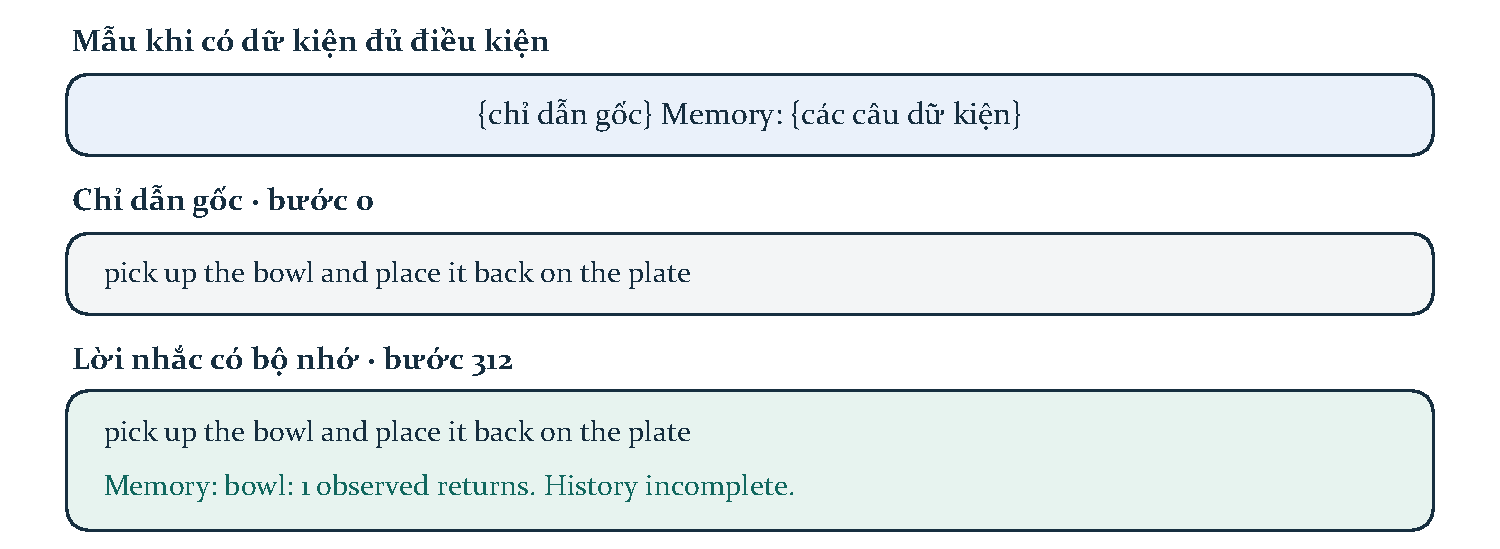
\includegraphics[width=.96\linewidth]{figures/loi-nhac-bo-nho.pdf}
\caption{Cấu trúc lời nhắc tích hợp bộ nhớ và ví dụ thực tế từ lượt chạy T1}
\label{fig:prompt-example}
\end{figure}

\label{sec:xvla-setup}

Để kiểm chứng tính tổng quát của phương pháp bộ nhớ sự kiện có bằng chứng theo RQ3, nghiên cứu triển khai song song quy trình thích ứng và đánh giá trên hai kiến trúc mô hình nền tiêu biểu: SmolVLA \cite{smolvla2025} và X-VLA \cite{xvla2025}. Bảng~\ref{tab:model-comparison} tổng hợp và so sánh chi tiết các thông số kỹ thuật và thiết lập điều khiển giữa hai mô hình. Trong khi SmolVLA dự đoán đoạn hành động độ dời tương đối $H = 50$ bước qua action expert nhỏ gọn, X-VLA dự đoán tư thế tuyệt đối 6D của đầu gắp với đoạn $H = 30$ bước qua 10 bước biến đổi Flow Matching trên nền tảng Florence-2. Cả hai mô hình đều vận hành ở nhịp truy vấn định kỳ $s = 10$ bước và chia sẻ cùng phân phối dữ liệu tinh chỉnh có bộ nhớ, với ngân sách thích ứng tham số lần lượt là 645.120 tham số LoRA trên SmolVLA và khoảng 11,87 triệu tham số trên X-VLA (5.000 bước huấn luyện, kích thước lô 32, tốc độ học $5\times10^{-5}$).

\begin{table}[htbp]
\centering\small
\caption{So sánh thông số kỹ thuật và thiết lập điều khiển giữa SmolVLA và X-VLA}
\label{tab:model-comparison}
\setlength{\tabcolsep}{4pt}
\begin{tabular}{>{\raggedright\arraybackslash}p{\dimexpr 0.28\textwidth-2\tabcolsep\relax}|>{\raggedright\arraybackslash}p{\dimexpr 0.36\textwidth-2\tabcolsep\relax}|>{\raggedright\arraybackslash}p{\dimexpr 0.36\textwidth-2\tabcolsep\relax}}
\toprule
\textbf{Thông số / Thuộc tính} & \textbf{SmolVLA} & \textbf{X-VLA} \\
\midrule
Checkpoint gốc & \texttt{lerobot/smolvla\_libero} & \texttt{2toINF/X-VLA-Libero} \\
Kiến trúc VLM & SigLIP + SmolLM2 & Florence-2-large \\
Không gian hành động & Độ dời tương đối 7D ($\Delta$ pose + kẹp) & Tư thế tuyệt đối 6D + kẹp \\
Bộ điều khiển robot & OSC (\textit{use\_delta} = True) ở 20 Hz & OSC (\textit{use\_delta} = False) ở 20 Hz \\
Đầu vào ảnh mô hình & $2 \times (256 \times 256)$ & $2 \times (224 \times 224)$ \\
Vector cảm nhận bản thể & 8D (vị trí, hướng xoay, kẹp) & 9D (vị trí, xoay 6D, kẹp; đệm) \\
Độ dài đoạn hành động ($H$) & 50 bước & 30 bước \\
Nhịp thực thi, truy vấn ($s$) & 10 bước định kỳ & 10 bước định kỳ \\
Tham số huấn luyện ($\phi$) & 645.120 tham số LoRA & $\sim 11{,}87$ triệu tham số \\
\bottomrule
\end{tabular}
\end{table}

Hiệu năng thực thi được lượng hóa qua ba chỉ số: chỉ số thành công toàn phần $S_i = \mathbf{1}[z_i = N \land P_i \land \neg O_i] \in \{0, 1\}$, trong đó $z_i$ là số chu kỳ xác nhận, $N$ là số chu kỳ yêu cầu, $P_i$ là vị từ kiểm tra đích, và $O_i$ là cờ vi phạm overshoot; tỷ lệ hoàn thành mốc $\mathrm{SCR}_i = z_i / N$; cùng tỷ lệ thành công thực nghiệm $\widehat{\mathrm{SR}} = \frac{1}{n}\sum_{i=1}^{n} S_i$ trên $n$ lượt đánh giá.

\section{Đối sánh vòng kín trên LIBERO-Mem}

Thực nghiệm trực tiếp với hai adapter F0 và F1 trên 20 trạng thái unseen của tác vụ một chu kỳ T1 và ba chu kỳ T3 cho thấy những sự khác biệt rõ rệt.
\begin{table}[htbp]
\centering\small
\caption{So sánh hiệu năng vòng kín giữa F0 và F1 trên SmolVLA và X-VLA (40 cặp unseen)}
\label{tab:e2-comparison}
\label{tab:e2-unseen-results}
\label{tab:xvla-e2-results}
\setlength{\tabcolsep}{4.5pt}
\begin{tabular}{l|l|l|r|r|r|r}
\toprule
\textbf{Kiến trúc} & \textbf{Tác vụ} & \textbf{Điều kiện} & \shortstack{\textbf{Thành công}\\\textbf{(SR)}} & \shortstack{\textbf{SCR}\\\textbf{trung bình}} & \shortstack{\textbf{Vi phạm}\\\textbf{overshoot}} & \shortstack{\textbf{Không đạt}\\\textbf{mốc nào}} \\
\midrule
SmolVLA & T1 & F0 & 3/20 & 0,250 & 2/20 & 15/20 \\
        &    & F1 & 0/20 & 0,050 & 1/20 & 19/20 \\
        & T3 & F0 & 1/20 & 0,167 & 0/20 & 15/20 \\
        &    & F1 & 0/20 & 0,033 & 0/20 & 18/20 \\
        \cmidrule{2-7}
        & \textbf{Tổng} & \textbf{F0} & \textbf{4/40} & \textbf{0,208} & \textbf{2/40} & \textbf{30/40} \\
        &               & \textbf{F1} & \textbf{0/40} & \textbf{0,042} & \textbf{1/40} & \textbf{37/40} \\
\midrule
X-VLA   & T1 & F0 & 0/20 & 0,500 & 10/20 & 10/20 \\
        &    & F1 & 0/20 & 0,600 & 12/20 & 8/20 \\
        & T3 & F0 & 0/20 & 0,200 & 1/20 & 10/20 \\
        &    & F1 & 0/20 & 0,383 & 4/20 & 8/20 \\
        \cmidrule{2-7}
        & \textbf{Tổng} & \textbf{F0} & \textbf{0/40} & \textbf{0,350} & \textbf{11/40} & \textbf{20/40} \\
        &               & \textbf{F1} & \textbf{0/40} & \textbf{0,492} & \textbf{16/40} & \textbf{16/40} \\
\bottomrule
\end{tabular}
\end{table}

Bảng~\ref{tab:e2-comparison} cho thấy các adapter của hai họ mô hình thất bại theo hai cách khác nhau. Trên SmolVLA, chênh lệch tỷ lệ thành công giữa F1 và F0 là $10$ điểm phần trăm, với khoảng bootstrap 95\% từ $-20$ đến $-2{,}5$ điểm phần trăm. F1 chỉ đạt SCR trung bình $0{,}042$ so với $0{,}208$ của F0, và 37 trong 40 lượt F1 không đạt mốc nào. Một cách giải thích khả dĩ là adapter LoRA khoảng 645 nghìn tham số khó điều kiện hóa cả thông tin ngữ cảnh của môi trường LIBERO lẫn LIBERO-Mem để đưa ra hành động, dẫn đến năng lực thao tác cơ sở sụt giảm nghiêm trọng trên cả 2 lượt huấn luyện, thể hiện qua tỉ lệ đạt subgoal SCR trung bình chỉ từ $0{,}04$ đến $0{,}2$. Ngoài ra, việc chạy module bộ nhớ đồng thời với mô hình điều khiển trên phần cứng phổ thông làm trung vị thời gian mỗi lượt tăng từ 213 giây lên 1.066 giây. Với mô phỏng chạy đồng bộ, độ trễ này không ảnh hưởng đến kết quả, nhưng sẽ là một thách thức khi triển khai thực tế.

Trên X-VLA, F1 tăng SCR trung bình thêm $0{,}142$ so với F0 (từ $0{,}350$ lên $0{,}492$), nhưng cả hai đều đạt 0/40 vì tại mọi lượt hoàn thành đủ chu kỳ, mô hình điều khiển tiếp tục thực hiện thêm một chu kỳ nữa và bị tính là overshoot. Như vậy, ở X-VLA vấn đề chính không nằm ở việc hoàn thành chu kỳ mà ở việc dừng đúng lúc. Hai mô hình khác nhau ở nhiều điểm, gồm kích thước, số tham số được tinh chỉnh, biểu diễn hành động và checkpoint gốc, nên nghiên cứu không quy sự khác biệt về kết quả cho riêng một yếu tố nào. Cơ chế can thiệp và hỗ trợ quyết định bằng bộ nhớ ở mục sau sẽ giúp xử lý trực tiếp vấn đề này.

\section{Kiểm tra thực thi chuỗi hành động và hiện tượng overshoot}
\label{sec:d2-evidence}
\label{sec:d2-calibration}

Phân tích các trường hợp thất bại từ thực nghiệm đối sánh vòng kín trên LIBERO-Mem cho thấy một nguyên nhân đáng chú ý: việc robot thực thi cố định toàn bộ đoạn hành động sinh ra từ chính sách có nguy cơ bám theo các quyết định đã lỗi thời khi môi trường vật lý đã chuyển pha thao tác. Cơ chế điều phối truy vấn theo sự kiện được đề xuất nhằm giải quyết vấn đề này. Bộ điều phối liên tục giám sát trạng thái bộ nhớ sự kiện; ngay khi xuất hiện biến cố chuyển tiếp vật lý có bằng chứng xác nhận, hệ thống chủ động ngắt đoạn hành động đang thực thi dở dang và kích hoạt mô hình VLA tái truy vấn sớm với ngữ cảnh ngôn ngữ cập nhật.

Hình~\ref{fig:smolvla-chunk-failure} minh họa một trường hợp thất bại điển hình của SmolVLA trên tác vụ T1 khi thực thi cố định đoạn hành động ở chế độ giám sát ngầm. Sau khi tiếp cận bát ở bước 110, robot tiếp tục thực thi chuỗi hành động mở đã hoạch định trước. Tuy nhiên, sai lệch tiếp xúc khiến bát trượt khỏi đầu kẹp tại bước 142. Do không có cơ chế ngắt sớm để tái truy vấn theo biến cố nhận thức, robot vẫn thực thi trọn vẹn quỹ đạo nâng lên, dẫn đến việc tay kẹp nâng rỗng lên không trung tại bước 240 trong khi bát vẫn nằm nguyên trên đĩa. Thất bại này làm nổi bật sự cần thiết của cơ chế điều phối linh hoạt, cho phép ngắt sớm chuỗi hành động khi xuất hiện bằng chứng chuyển pha vật lý để tái lập kế hoạch kịp thời.

\begin{figure}[H]
\centering
\includegraphics[width=\linewidth]{figures/smolvla-chunk-failure.png}
\caption{Chuỗi hành vi thất bại của SmolVLA khi thực thi đoạn hành động}
\label{fig:smolvla-chunk-failure}
\end{figure}

Để kiểm chứng tính đúng đắn và hiệu quả của cơ chế này theo RQ2, nghiên cứu thiết lập thực nghiệm đối đầu trực tiếp giữa hai chế độ điều phối. Ở chế độ giám sát ngầm, bộ điều phối chỉ thụ động ghi nhận sự kiện vào bộ nhớ mà không can thiệp vào chu kỳ điều khiển, duy trì nghiêm ngặt nhịp truy vấn định kỳ $s = 10$ bước. Ngược lại, ở chế độ theo sự kiện, bộ điều phối được cấp quyền ngắt sớm đoạn hành động ngay khi có bằng chứng sự kiện mới để gọi lại chính sách trước hạn.

Quy trình đánh giá được thực hiện đồng nhất trên cả hai kiến trúc mô hình với cùng seed 42, khảo sát 12 trạng thái seen thuộc nhóm phát triển trên cả hai tác vụ T1 và T3. Với mỗi mô hình, thực nghiệm gồm 24 lượt ở chế độ theo sự kiện đối đầu ghép cặp với 24 lượt ở chế độ giám sát ngầm, tương ứng 48 lượt chạy vòng kín độc lập cho từng kiến trúc và tổng cộng 96 lượt đánh giá. Bảng~\ref{tab:d2-combined} tổng hợp kết quả đối sánh chi tiết giữa hai chế độ trên cả hai mô hình.

\begin{table}[htbp]
\centering\footnotesize
\caption{Đánh giá cơ chế truy vấn theo sự kiện và hiện tượng overshoot trên SmolVLA và X-VLA}
\label{tab:d2-combined}
\label{tab:d2-decision-results}
\label{tab:d2-calibration-results}
\setlength{\tabcolsep}{3.5pt}
\begin{tabular}{l|l|l|r|r|r|r|r}
\toprule
\textbf{Mô hình} & \textbf{Tác vụ} & \textbf{Chế độ} & \shortstack{\textbf{Thành}\\\textbf{công}} & \shortstack{\textbf{SCR}\\\textbf{TB}} & \shortstack{\textbf{Vi phạm}\\\textbf{overshoot}} & \shortstack{\textbf{Lần gọi}\\\textbf{VLA/lượt}} & \shortstack{\textbf{Lượt có}\\\textbf{gọi sớm}} \\
\midrule
SmolVLA & T1 & Giám sát & 1/12 & 0,167 & 1/12 & 94,33 & 0/12 \\
        &    & Theo sự kiện & 1/12 & 0,250 & 2/12 & 97,75 & 11/12 \\
        \cmidrule{2-8}
        & T3 & Giám sát & 0/12 & 0,056 & 0/12 & 100,00 & 0/12 \\
        &    & Theo sự kiện & 0/12 & 0,083 & 0/12 & 102,00 & 11/12 \\
\midrule
X-VLA   & T1 & Giám sát & 0/12 & 0,917 & 11/12 & 24,83 & 0/12 \\
        &    & Theo sự kiện & 0/12 & 0,833 & 10/12 & 31,92 & 11/12 \\
        \cmidrule{2-8}
        & T3 & Giám sát & 0/12 & 0,583 & 5/12 & 73,50 & 0/12 \\
        &    & Theo sự kiện & 0/12 & 0,528 & 4/12 & 78,00 & 11/12 \\
\bottomrule
\end{tabular}
\end{table}

Số liệu tại Bảng~\ref{tab:d2-combined} cho thấy cơ chế theo sự kiện vận hành hoàn toàn nhất quán về mặt kỹ thuật trên cả hai kiến trúc. Trên mỗi mô hình, có đúng 22 trên 24 lượt chạy ghi nhận ít nhất một lần kích hoạt ngắt sớm, gồm 11 trên 12 lượt ở tác vụ T1 và 11 trên 12 lượt ở tác vụ T3. Toàn bộ các lần gọi sớm này, gồm 56 lần ở SmolVLA và 70 lần ở X-VLA, đều xuất phát từ bằng chứng sự kiện mới được xác thực, chứng minh bộ điều phối phản ứng chính xác theo biến cố nhận thức thời gian thực chứ không kích hoạt ngẫu nhiên. Số lần gọi chính sách trung bình mỗi lượt ở chế độ theo sự kiện tăng nhẹ tương ứng với các thời điểm ngắt đoạn hành động trước hạn.

Mặc dù cơ chế ngắt sớm vận hành đúng thiết kế, tác động thực tế lên hiệu năng điều khiển vòng kín lại bộc lộ những đặc tính đối lập rõ rệt giữa hai họ mô hình:

Đối với SmolVLA, việc ngắt sớm đoạn hành động giúp cải thiện nhẹ tỷ lệ hoàn thành mốc SCR, tăng từ 0,167 lên 0,250 ở tác vụ T1 và từ 0,056 lên 0,083 ở tác vụ T3. Tuy nhiên, tỷ lệ thành công toàn phần không có sự bứt phá, duy trì ở mức 1 trên 12 lượt ở tác vụ T1 và 0 trên 12 lượt ở tác vụ T3 trên cả hai chế độ. Lượt T1 trạng thái 7 thành công ở bước 409 được minh họa tại Hình~\ref{fig:libero-mem-d2-t1-success} là một ví dụ trực quan đối lập với trường hợp thất bại ở Hình~\ref{fig:smolvla-chunk-failure}, cho thấy việc tái truy vấn đúng lúc giúp robot hoàn thành chuỗi thao tác kẹp nhấc và đặt bát. Dù vậy, việc ngắt sớm chỉ tối ưu hóa thời điểm cập nhật ngữ cảnh chứ không thể bù đắp được sự suy giảm năng lực vận động cơ sở sau thích ứng LoRA trên SmolVLA F1.

Trái ngược với SmolVLA, X-VLA thể hiện năng lực thao tác vật lý vượt trội khi đạt tỷ lệ hoàn thành mốc SCR rất cao ở cả hai chế độ, đạt từ 0,833 đến 0,917 ở tác vụ T1 và từ 0,528 đến 0,583 ở tác vụ T3. Tuy vậy, tỷ lệ thành công toàn phần của X-VLA vẫn là 0 trên 24 lượt ở cả hai chế độ. Nguyên nhân trực tiếp là phần lớn các lượt chạy đều thất bại do vi phạm lỗi overshoot. Sau khi hoàn thành thao tác đặt bát vào đĩa, mô hình tiếp tục quán tính sinh chuỗi hành động tiếp cận mới cho đến khi môi trường kết thúc lượt chạy. Ngay cả khi được ngắt action chunk và cho quan sát state mới, chính sách không phân biệt được trạng thái bắt đầu khi chưa thực hiện hành động và trạng thái kết thúc khi đã hoàn thành đủ lượt gắp.

\begin{figure}[H]
\centering
\includegraphics[width=\linewidth]{figures/t1-truy-van-som.png}\par
{\small\makebox[.25\linewidth]{Bước 0}%
\makebox[.25\linewidth]{Bước 142}%
\makebox[.25\linewidth]{Bước 409}%
\makebox[.25\linewidth]{Bước 1.000}\par}
\caption{Chuỗi hành vi của lượt T1 thành công khi kích hoạt truy vấn sớm}
\label{fig:libero-mem-d2-t1-success}
\end{figure}

\label{sec:xvla-d2-cohort}

Kết quả đối sánh vòng kín cùng thí nghiệm ngắt chuỗi hành động và truy vấn sớm trên cả hai mô hình giúp ta rút ra được một số quan sát: Việc ngắt chuỗi hành động action chunk và kích hoạt truy vấn sớm có thể tạo ra những đóng góp ý nghĩa nhất định, bằng chứng nằm ở cặp lượt chuyển từ False thành True tại task T1 state 7. Tuy nhiên việc ngắt sớm đoạn hành động và chuyển tiếp trạng thái cũng có thể thất bại, như state 5 của task T1 chuyển từ True sang False. Một quan sát khác là chỉ dẫn \texttt{Memory:...} không mang tính cưỡng chế để buộc chính sách VLA dừng lại khi đã hoàn thành nhiệm vụ. Bên cạnh đó, kết quả đo độ trễ của bộ ghi thị giác cho thấy độ trễ trung vị giữa thời điểm xác nhận được sự kiện và thời điểm diễn ra thực tế dao động từ 7 bước đến hàng chục bước, khiến thông tin ngôn ngữ luôn đến muộn hơn động học thực tế của robot và thay đổi của môi trường.

Ngoài ra, khảo sát ngoại tuyến trên các logged trace xác nhận việc nén ngân sách token xuống mức hai phần ba không làm suy hao dữ kiện bộ nhớ so với mức đầy đủ $B = 48$ token, với độ dài lời nhắc trung bình là 21 token ở tác vụ T1 và 26 token ở tác vụ T3. Khi rút xuống mức một phần ba, chỉ còn 35\% truy vấn ở T1 và 5,7\% truy vấn ở T3 giữ được dữ kiện. Vì mức hai phần ba và mức đầy đủ cho cùng kết quả truyền đạt dữ kiện, ngân sách $B = 48$ token không tạo ra điểm nghẽn biểu diễn trên các tác vụ khảo sát.

Sự hạn chế của chỉ dẫn ngôn ngữ trong việc ngăn chặn lỗi overshoot trên X-VLA là động lực trực tiếp dẫn đến thiết kế cơ chế hỗ trợ dừng thao tác dựa trên bộ nhớ được trình bày chi tiết tại Mục~\ref{sec:memory-halt}.

\section{Dừng thực thi dựa trên bộ nhớ trên X-VLA}
\label{sec:memory-halt}

Hiện tượng overshoot liên tục trên X-VLA cho thấy chính sách không có tín hiệu dừng sau khi hoàn thành nhiệm vụ. Thực nghiệm này sẽ khảo sát khả năng sử dụng bằng chứng từ bộ nhớ làm tín hiệu dừng ngoại vi. Quy trình sẽ bao gồm: đo độ nhạy của các phiên bản bộ nhớ trong việc phát hiện sự kiện, phân tích thời điểm dừng của quỹ đạo, và mô phỏng trạng thái giữ yên sau khi dừng. Các kết quả đều được ghi nhận và đo đạc theo giao thức riêng của nghiên cứu và mang tính mô tả, không so sánh trực tiếp với performance của tác giả.

\label{sec:writer-recall}
Để đánh giá độ nhạy phát hiện sự kiện, nghiên cứu phân tích 35 mốc hoàn thành chu kỳ được xác nhận trên toàn bộ 40 quỹ đạo F1 đã ghi ở thực nghiệm E2, gồm 20 lượt tác vụ T1 và 20 lượt tác vụ T3. Trong 40 lượt này, có 16 lượt hoàn thành trọn vẹn số chu kỳ mục tiêu của nhiệm vụ, gồm 12 lượt ở tác vụ T1 và 4 lượt ở tác vụ T3; các lượt T3 còn lại đóng góp thêm các lượt đạt mốc chu kỳ trung gian SCR, đưa tổng số mốc chu kỳ thành công lên 35 mốc. Nghiên cứu đối chiếu ba phiên bản bộ ghi thị giác gồm V1 dùng quy tắc cơ sở, V3 bổ sung kiểm tra chuyển động, V4 tích hợp thêm vị trí đĩa đích, cùng tín hiệu proprioception chạm đáy được trích xuất trực tiếp từ vị trí và độ mở của đầu gắp theo định nghĩa tại Mục~\ref{sec:method-memory-halt}.

\begin{table}[htbp]
\centering\small
\caption{Độ phủ mốc trên E2 của X-VLA (35 mốc, sai lệch $\pm 20$ bước) và trên nhóm phát triển}
\label{tab:xvla-writer-recall}
\setlength{\tabcolsep}{4pt}
\begin{tabular}{l|r|r|r|r|r}
\toprule
& \multicolumn{4}{c}{\textbf{Tập đánh giá}} & \textbf{Tập phát triển} \\
\cmidrule(lr){2-5}\cmidrule(lr){6-6}
\textbf{Nguồn} & \textbf{TP} & \textbf{FP} & \textbf{FN} & \textbf{Covarage} & \textbf{Covarage} \\
\midrule
V1 & 7 & 5 & 28 & 20\% & 49\% \\
V3 & 6 & 3 & 29 & 17\% & 50\% \\
V4 & 7 & 3 & 28 & 20\% & 65\% \\
Tín hiệu proprioception & 18 & 4 & 17 & 51\% & 96\% \\
V4 + proprioception  & 20 & 6 & 15 & 57\% & 99\% \\
\bottomrule
\end{tabular}
\par\smallskip
{\footnotesize Nhóm phát triển: 394 mốc của 198 quỹ đạo mẫu tác giả. Phủ = đúng/mốc.\par}
\end{table}

Bảng~\ref{tab:xvla-writer-recall} cho thấy hợp nhất bộ ghi thị giác với tín hiệu proprioception nâng độ phủ lên $57{,}1$\% trên tập đánh giá (20/35 mốc; khoảng Wilson 95\% từ $40{,}8$\% đến $72{,}0$\%), so với khoảng $20$\% của bộ ghi thị giác đứng riêng; ở tập phát triển, tín hiệu proprioception đạt $96$\% và bản hợp nhất đạt $99$\%. Hai nguồn bổ trợ nhau một cách rất tinh tế vì tín hiệu proprioception không phụ thuộc vào việc bát có che khuất đĩa đích hay không và phát hiện sự kiện nhấc, hạ với latency = 0, còn bộ ghi thị giác bắt được một số lượt nhấc thấp mà ngưỡng proprioception bỏ lỡ. Cách hợp nhất theo từng chu kỳ lấy phép hợp của hai nguồn. Độ phủ trên quỹ đạo do mô hình tạo vẫn thấp hơn nhiều so với trên demo con người điều khiển. Điều này phản ánh việc quỹ đạo X-VLA sinh có những sai khác về phong cách chuyển động so với dữ liệu quy đạo của con người. Trong 17 mốc mà tín hiệu proprioception bỏ sót, 11 mốc có độ nhấc thấp dưới 8~cm, 3 mốc có điểm chạm đáy cao hơn ngưỡng cho phép, 1 mốc không có pha kẹp và 2 mốc có hành vi nhấc xảy ra trước mốc. Nguyên nhân khiến bộ ghi thị giác chỉ đạt khoảng $20$\% chưa được tách riêng; che khuất thị giác là một giả thuyết hợp lý nhưng hiện chưa đưa vào phạm vi nghiên cứu hiện tại.

\label{sec:halt-timing}
\label{sec:halt-forks}
Cơ chế dừng dựa trên bộ nhớ được đánh giá tại mỗi ranh giới truy vấn theo quy tắc trình bày tại Mục~\ref{sec:method-memory-halt}: hệ thống chủ động ngắt thực thi khi bộ nhớ ghi nhận đủ số chu kỳ mục tiêu và tay kẹp đã mở, sau đó chốt trạng thái và duy trì mở kẹp giữ yên. Quyết định dừng được gọi là kịp lúc nếu diễn ra sau mốc hoàn thành và trước khi xuất hiện overshoot, và gọi là dừng sớm nếu diễn ra trước khi đạt mốc hoàn thành. Do quyết định dừng chỉ phụ thuộc vào lịch sử đã qua theo nguyên tắc nhân quả, vector các hành động trước bước dừng có giá trị đúng bằng quỹ đạo gốc. Phương pháp mô phỏng can thiệp dừng tái lập môi trường về trạng thái ban đầu, phát lại hành động đã ghi tới thời điểm dừng, rồi kích hoạt trạng thái giữ yên cho tới khi kết thúc lượt chạy.

\begin{table}[htbp]
\centering\small
\caption{Thời điểm dừng và tỉ lệ thành công toàn phần trên 40 lượt X-VLA F1}
\label{tab:halt-combined}
\label{tab:halt-timing-combined}
\label{tab:halt-forks-combined}
\setlength{\tabcolsep}{3pt}
\begin{tabular}{>{\raggedright\arraybackslash}p{.37\textwidth}|r|r|r|r|r|r}
\toprule
& \multicolumn{2}{c|}{\textbf{Thời điểm dừng}} & \multicolumn{4}{c}{\textbf{Thành công toàn phần}} \\
\cmidrule(lr){2-3}\cmidrule(lr){4-7}
\textbf{Nguồn quyết định dừng} & \shortstack{\textbf{Kịp}\\\textbf{lúc}} & \shortstack{\textbf{Dừng}\\\textbf{sớm}} & \shortstack{\textbf{Tổng}\\\textbf{(40)}} & \shortstack{\textbf{T1}\\\textbf{(20)}} & \shortstack{\textbf{T3}\\\textbf{(20)}} & \shortstack{\textbf{$p$ hai}\\\textbf{phía}} \\
\midrule
Chỉ bộ ghi thị giác V4 & 6 & 0 & 5 & 5 & 0 & 0,063 \\
Chỉ tín hiệu proprioception & 6 & 2 & 7 & 7 & 0 & 0,016 \\
Kết hợp, có chặn bằng thị giác & 6 & 0 & 5 & 5 & 0 & 0,063 \\
\textbf{Kết hợp hai nguồn} & 9 & 2 & 9 & 9 & 0 & 0,004 \\
\midrule
Kết hợp hai nguồn, chạy vòng kín & 9 & 2 & 9 & 8 & 1 & 0,004 \\
\bottomrule
\end{tabular}
\par\smallskip
\end{table}

\label{sec:halt-vs-prior}
Bảng~\ref{tab:halt-combined} cho thấy việc kết hợp bộ ghi thị giác V4 với tín hiệu proprioception nâng số lượt thành công mô phỏng từ 0/40 lên 9/40. Gap còn lại chủ yếu nằm ở khả năng phối hợp thao tác của mô hình và các edge case của những lượt overshoot xảy ra ngay trong đoạn hành động ranh giới. Việc cộng hai nguồn theo từng chu kỳ giúp tăng số lần dừng kịp lúc từ 6 lên 9, đổi lại có hai lần dừng sớm. Ngược lại, khi dùng thị giác để chặn các quyết định dừng của tín hiệu proprioception thì không còn dừng sớm, nhưng số lần dừng kịp lúc quay về 6 và thành công giảm xuống 5/40, vì thị giác thường chưa xác nhận được mốc ở những lượt quan trọng. Trên T3, mô phỏng can thiệp dừng cho 0/20 ở mọi nguồn vì chính sách hiếm khi hoàn thành đủ ba chu kỳ, nhưng khi chạy vòng kín thật có 1/20 lượt thành công.

Phương pháp mô phỏng can thiệp dừng tái hiện trung thực kết quả cuối cùng trên 7 trong 8 lượt kiểm tra, dù quỹ đạo phát lại lệch nhau từ dưới một milimét đến khoảng hai centimet. Để kiểm chứng, cấu hình kết hợp hai nguồn được chạy lại vòng kín thật trên cùng 40 trạng thái. Kết quả đạt 9/40 thành công, và bước dừng trùng khớp với thí nghiệm mô phỏng ở cả 40 lượt: cả 9 lượt dừng kịp lúc đều thành công, cả hai lượt dừng sớm (T1 trạng thái 4 và 16) đều thất bại. Phân bổ theo tác vụ khác mô phỏng ở hai lượt: T1 trạng thái 4, vốn có độ lệch quỹ đạo 1,75~cm tại bước dừng, thành công trong mô phỏng nhưng thất bại khi chạy thật; T3 trạng thái 15 thất bại trong mô phỏng nhưng thành công khi chạy thật, là lượt T3 thành công duy nhất của X-VLA trên E2. Do đó kết quả T3 không phải luôn bằng 0 như mô phỏng cho thấy, nhưng vì chỉ có một lượt nên đây là bằng chứng về khả năng xảy ra chứ không phải một tỷ lệ. Tính ổn định của quy tắc dừng sẽ được kiểm chứng độc lập trên một tập trạng thái chưa biết như trình bày dưới đây.

Để tách phần lợi ích do bản thân việc dừng mang lại, nghiên cứu thay thời điểm dừng bằng các thời điểm ngẫu nhiên: một ranh giới truy vấn ngẫu nhiên, một ranh giới ngẫu nhiên có tay kẹp đang mở, và các bước cố định 100, 150, 200, với ba lần rút cho mỗi kiểu ngẫu nhiên, tổng cộng 28 lượt mô phỏng can thiệp dừng. Các điều kiện này đạt 1--5/40 thành công, trung bình $3{,}7/40$, và không điều kiện nào đạt 9/40. Như vậy một phần thành công đến từ việc chỉ cần dừng trong khoảng 7--50 bước giữa lúc hoàn thành và lúc overshoot, còn bằng chứng bộ nhớ nâng tỷ lệ này từ khoảng 4/40 lên 9/40.

\label{sec:halt-seen12}

Khóa luận cũng thực hiện so sánh cơ chế can thiệp dừng trên cầu hình tương từ, chạy vòng kín trên 12 trạng thái, ghép cặp với lượt không dừng cùng seed. Các trạng thái này chưa được dùng để chọn cấu hình dừng, nên kết quả kiểm chứng quy tắc dừng chứ không kiểm chứng khả năng điều khiển tổng quát của chính sách.

\begin{table}[htbp]
\centering\small
\caption{Cơ chế dừng trên 12 trạng thái của X-VLA F1}
\label{tab:halt-seen12}
\begin{tabular}{l|r|r|r|r|r}
\toprule
\textbf{Điều kiện} & \textbf{Hoàn thành} & \textbf{Dừng kịp lúc} & \textbf{Dừng sớm} & \textbf{T1} & \textbf{T3} \\
\midrule
Không dừng & 8/12 & -- & -- & 0/6 & 0/6 \\
Có dừng & 8/12 & 6 & 0 & 5/6 & 1/6 \\
\bottomrule
\end{tabular}
\par\smallskip
{\footnotesize *Hoàn thành: đạt số chu kỳ mục tiêu.\par}
\end{table}

Không dừng đạt 0/12 vì cả 8 lượt hoàn thành đều overshoot; có dừng đạt 6/12 (khoảng Wilson 95\%: 25--75\%), với 6 cặp có lợi, 0 cặp bất lợi và 6 cặp trung tính, $p = 0{,}031$ theo kiểm định dấu chính xác hai phía. Cơ chế dừng chuyển 6 trong 8 lượt hoàn thành nhưng overshot sang thành công, so với 9 trong 16 trên E2; hai lượt bỏ lỡ overshoot sớm nên không bắt được. Không có lượt dừng sớm nào, và bốn lượt T3 chưa hoàn thành giữ nguyên tỷ lệ hoàn thành mốc. Với 12 cặp, kết quả mang tính thăm dò nhiều hơn nhưng cũng phần nào củng cố cho lợi ích mà cơ chế dừng hành động mang lại.

\section{Can thiệp triệt tiêu bộ nhớ tại một truy vấn}
\label{sec:e45-one-query}

Nhằm kiểm chứng tính nhân quả ở tầng quyết định cục bộ của RQ1, nghiên cứu thực hiện can thiệp xóa bỏ truy vấn then chốt trên ba ca đại diện: hai lượt thành công của SmolVLA tại bước 142 của trạng thái 7 và bước 10 của trạng thái 5, cùng một lượt X-VLA thất bại, kéo dài 1.000 bước, tại bước 10 của trạng thái 10. Mỗi ca được phân tách thành nhánh đối chứng giữ nguyên lời nhắc gốc và nhánh can thiệp loại bỏ hoàn toàn thành phần văn bản bộ nhớ tại bước chỉ định, trong khi toàn bộ quan sát và hành động trước thời điểm can thiệp được tái lập trùng khớp tuyệt đối.

\begin{table}[htbp]
\centering\small
\caption{Kết quả can thiệp triệt tiêu bộ nhớ tại một truy vấn trên SmolVLA và X-VLA}
\label{tab:e45-one-query}
\setlength{\tabcolsep}{3.5pt}
\begin{tabular}{l|r|r|r|c|l}
\toprule
\textbf{Nhánh thử nghiệm} & \shortstack{\textbf{Số bước}\\\textbf{trùng gốc}} & \shortstack{\textbf{Sai khác $L_2$}\\\textbf{bước đầu}} & \shortstack{\textbf{Sai khác $L_2$}\\\textbf{đoạn thực thi}} & \textbf{SCR} & \textbf{Kết quả} \\
\midrule
\multicolumn{6}{l}{\textbf{Ca 1: SmolVLA, trạng thái 7, điểm can thiệp $t^* = 142$ }} \\
\midrule
Đối chứng & 1.000 / 1.000 & 0,000 & 0,000 & 1,0 & Thành công \\
Can thiệp & 142 / 1.000   & 0,188 & 0,529 & 0,0 & Thất bại \\
\midrule
\multicolumn{6}{l}{\textbf{Ca 2: SmolVLA, trạng thái 5, điểm can thiệp $t^* = 10$ }} \\
\midrule
Đối chứng & 1.000 / 1.000 & 0,000 & 0,000 & 1,0 & Thành công \\
Can thiệp & 10 / 1.000    & 0,150 & 0,618 & 0,0 & Thất bại \\
\midrule
\multicolumn{6}{l}{\textbf{Ca 3: X-VLA, trạng thái 10, điểm can thiệp $t^* = 10$}} \\
\midrule
Đối chứng & 1.000 / 1.000 & 0,000 & 0,000 & 0,0 & Thất bại \\
Can thiệp & 10 / 1.000    & 0,009 & 0,043 & 0,0 & Thất bại \\
\bottomrule
\end{tabular}
\par\smallskip
\end{table}

Bảng~\ref{tab:e45-one-query} cho thấy ở cả ba ca, nhánh đối chứng giữ nguyên lời nhắc đã tái lập chính xác 1.000 trên 1.000 hành động của quỹ đạo gốc. Ngược lại, nhánh can thiệp bị triệt tiêu đoạn văn bản bộ nhớ bắt đầu rẽ nhánh ngay tại thời điểm can thiệp, khiến số bước trùng khớp với quỹ đạo gốc dừng lại ở bước 142 và bước 10. Mức độ sai khác hành động được định lượng qua chuẩn khoảng cách Euclidean $L_2$ giữa vector hành động của nhánh can thiệp so với nhánh đối chứng, xét tại bước đầu tiên và trung bình tích lũy trên toàn bộ đoạn 10 hành động được bộ điều khiển thực thi. Trên SmolVLA, sai khác $L_2$ tại bước đầu đạt $0{,}188$ và $0{,}150$, dẫn đến việc cả hai lượt vốn hoàn thành tác vụ đều rớt về điểm số SCR bằng 0 và kết thúc do hết thời gian. Trên X-VLA, sai khác $L_2$ chỉ đạt $0{,}009$ và nhánh đối chứng vốn cũng thất bại, nên can thiệp không làm đảo chiều kết quả cuối cùng.

Các phép thử cục bộ này khẳng định chính sách SmolVLA có độ nhạy cao đối với sự hiện diện của thành phần văn bản bộ nhớ tại từng thời điểm suy luận. Tuy nhiên, sự biến đổi hành động này chưa đủ cơ sở để kết luận mô hình đã thực sự hiểu ngữ nghĩa của thông tin ghi nhớ, bởi việc cắt bỏ toàn bộ chuỗi ký tự cũng đồng thời làm biến đổi độ dài chuỗi token đầu vào của mô hình ngôn ngữ. Bên cạnh đó, hai ca SmolVLA được trích xuất từ nhóm các quỹ đạo hiếm hoi thành công và cả ba trường hợp đều mang tính chẩn đoán vi mô, không thể coi là đại diện cho phân phối toàn cục trên không gian trạng thái.

\section{Đánh giá duy trì kỹ năng cơ sở trên LIBERO-10}
\label{sec:e6-retention}

Để khảo sát năng lực được giữ lại sau khi huấn luyện trên miền tác vụ mới, khóa luận so sánh ba điều kiện B0, F0 và F1-off trên 10 tác vụ thuộc LIBERO-10, mỗi tác vụ 5 trạng thái khởi tạo, tạo thành 50 bộ ba ghép cặp cho mỗi mô hình. Cả ba điều kiện dùng cùng 50 trạng thái khởi tạo và cùng seed cho từng lượt, và đều chạy ở chế độ tắt bộ nhớ, tức chính sách chỉ nhận chỉ dẫn gốc. Nhờ đó, so sánh F0 với B0 phản ánh ảnh hưởng của việc tinh chỉnh nói chung, còn so sánh F1-off với F0 phản ánh phần khác biệt gắn với việc huấn luyện trên lời nhắc có bộ nhớ, vì hai adapter dùng cùng dữ liệu và ngân sách cập nhật như mô tả ở Chương~3. Thử nghiệm nhằm xác định liệu mô hình có gặp hiện tượng quên thảm khốc sau quá trình tinh chỉnh tham số hay không.

\begin{table}[htbp]
\centering\small
\caption{Tổng hợp mức độ duy trì và phân rã suy giảm kỹ năng cơ sở trên LIBERO-10}
\label{tab:e6-retention-combined}
\label{tab:e6-retention-results}
\label{tab:xvla-e6-results}
\setlength{\tabcolsep}{4pt}
\begin{tabular}{l|l|c|r|c|c|>{\raggedright\arraybackslash}p{4.2cm}}
\toprule
\textbf{Kiến trúc} & \textbf{Điều kiện} & \textbf{Thành công} & \textbf{Tỉ lệ} & $\mathbf{\Delta}$ \textbf{vs B0} & $\mathbf{\Delta}$ \textbf{vs F0} & \textbf{Mức độ duy trì kỹ năng} \\
\midrule
SmolVLA & B0     & 37/50 & 74{,}0\% & —        & —        & Chuẩn cơ sở \\
        & F0     & 32/50 & 64{,}0\% & $-10{,}0\%$ & —        & Giảm nhẹ do tinh chỉnh \\
        & F1-off & 23/50 & 46{,}0\% & $-28{,}0\%$ & $-18{,}0\%$ & Suy giảm mạnh ở tiếp xúc tinh vi \\
\midrule
X-VLA   & B0     & 47/50 & 94{,}0\% & —        & —        & Chuẩn cơ sở \\
        & F0     & 44/50 & 88{,}0\% & $-6{,}0\%$  & —        & Duy trì ổn định \\
        & F1-off & 46/50 & 92{,}0\% & $-2{,}0\%$  & $+4{,}0\%$  & Giữ trọn vẹn kỹ năng cơ sở \\
\bottomrule
\end{tabular}
\end{table}

Bảng~\ref{tab:e6-retention-combined} cho thấy trên SmolVLA, điều kiện F1-off suy giảm 28 điểm phần trăm so với mô hình gốc B0 khi tỉ lệ thành công giảm từ 37/50 xuống 23/50, đồng thời thấp hơn điều kiện F0 18 điểm phần trăm. Trong khi đó, F0 đạt 32/50 lượt thành công, chỉ giảm nhẹ 10 điểm phần trăm so với B0. Vì cả ba điều kiện đều không nhận đoạn văn bản bộ nhớ khi suy luận trên LIBERO-10, các mức chênh lệch này phản ánh tác động trực tiếp từ sự biến đổi trọng số sau quá trình tinh chỉnh. Việc thiết lập điều kiện đối chứng F0 cho phép bóc tách hai thành phần suy thoái: phần lớn mức sụt giảm hiệu năng của F1-off nằm ở khoảng cách giữa F0 và F1-off, tức gắn liền với việc huấn luyện trên phân phối dữ liệu có lời nhắc bộ nhớ hơn là do bản thân quá trình tinh chỉnh tham số. Các tác vụ đòi hỏi căn chỉnh tiếp xúc tinh vi chịu ảnh hưởng nặng nề nhất. Điển hình ở tác vụ đặt sách vào hộp được minh họa tại Hình~\ref{fig:e6-book-placement}, mô hình gốc B0 hoàn thành toàn bộ 5/5 lượt thử, nhưng F0 chỉ đạt 1/5 và F1-off thất bại hoàn toàn ở cả 5 lượt. Trong trường hợp này, cánh tay robot vẫn nhấc được sách lên khỏi mặt bàn nhưng không thể đặt chính xác vào hộp chứa. Ngược lại, ở tác vụ thao tác đóng mở đơn giản như tác vụ 3, cả ba điều kiện đều duy trì trọn vẹn 5/5 lượt thành công.

\begin{figure}[H]
\centering
\includegraphics[width=.96\linewidth]{figures/e6-dat-sach.png}\par
{\small\makebox[.24\linewidth]{Khung 0}%
\makebox[.24\linewidth]{Khung 77}%
\makebox[.24\linewidth]{Khung 103}%
\makebox[.24\linewidth]{Khung 1.000}\par}
\caption{Quá trình SmolVLA F1-off nhấc sách nhưng không thể đặt vào hộp ở tác vụ 5}
\label{fig:e6-book-placement}
\end{figure}

Đối với X-VLA, khả năng duy trì kỹ năng cơ sở thể hiện tính ổn định vượt trội. Điều kiện F1-off đạt 46/50 lượt thành công, tương đương mức 47/50 của mô hình cơ sở B0, trong khi F0 đạt 44/50 lượt. Hiệu năng của cả hai adapter đều duy trì sát mốc chuẩn ban đầu và không ghi nhận hiện tượng suy thoái kỹ năng đáng kể. Sự tương phản này cho thấy các mô hình có dung lượng tham số lớn cùng biểu diễn hành động tư thế tuyệt đối có khả năng bảo toàn không gian kỹ năng ban đầu tốt hơn trước các can thiệp tinh chỉnh thích ứng. Hình~\ref{fig:e6-retention-by-task} đối chiếu trực quan số lượt thành công trên từng tác vụ của ba điều kiện B0, F0 và F1-off trên cả hai kiến trúc, làm rõ sự tương phản giữa mức độ suy giảm kỹ năng cục bộ của SmolVLA và tính ổn định bền vững của X-VLA.

\begin{figure}[H]
\centering
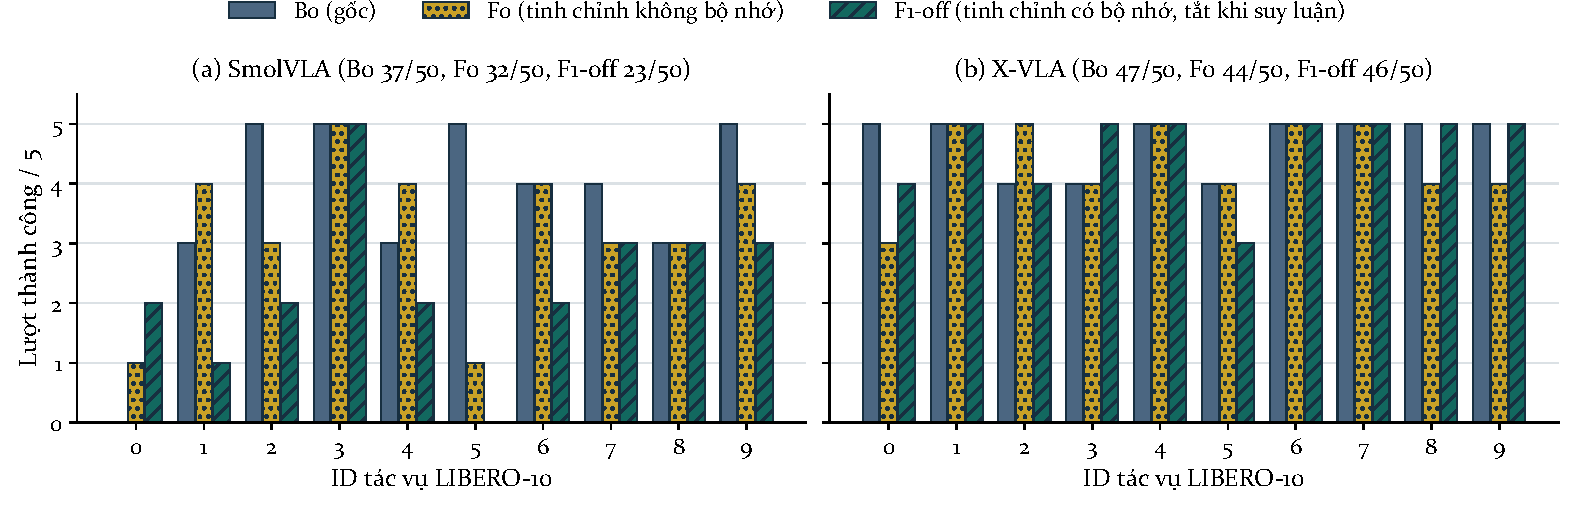
\includegraphics[width=.96\linewidth]{figures/duy-tri-e6.pdf}
\caption{Số lượt thành công theo từng tác vụ LIBERO-10 của B0, F0 và F1-off trên SmolVLA và X-VLA}
\label{fig:e6-retention-by-task}
\end{figure}

\section{Tổng hợp kết quả theo câu hỏi nghiên cứu}
\label{sec:ch4-rq-summary}

\textbf{RQ1: Giá trị của bộ nhớ sự kiện.} Đánh giá vòng kín cho thấy việc đưa dữ kiện bộ nhớ vào lời nhắc ngôn ngữ tác động trực tiếp đến động học ra quyết định nhưng chưa đủ để tự động nâng cao tỷ lệ thành công nếu thiếu cơ chế kiểm soát chu kỳ. Trên SmolVLA, F1 đạt 0 trên 40 lượt so với 4 trên 40 lượt của F0; trên X-VLA, cả hai cấu hình đạt 0 trên 40 lượt do lỗi lặp thao tác thừa, mặc dù F1 đạt tỷ lệ hoàn thành mốc SCR cao hơn rõ rệt với $0{,}492$ so với $0{,}350$. Thử nghiệm can thiệp triệt tiêu tại một truy vấn khẳng định chính sách nhạy bén ở mức cục bộ với sự hiện diện của đoạn văn bản ghi nhớ. Giá trị thực tế then chốt của bộ nhớ sự kiện được thể hiện rõ nét khi đóng vai trò nguồn bằng chứng định lượng cho cơ chế dừng ngoại vi: khi thay thế bằng các thời điểm dừng ngẫu nhiên, số lượt hoàn thành tác vụ sụt giảm mạnh từ 9 lượt xuống mức trung bình $3{,}7$ trên 40 lượt.

\textbf{RQ2: Độ tin cậy của bằng chứng và hiệu quả của cơ chế dừng.} Nghiên cứu đã chứng minh tính khả thi và hiệu quả rõ rệt của cơ chế điều phối theo sự kiện cùng giải pháp can thiệp dừng dựa trên bằng chứng bộ nhớ. Trong điều khiển vòng kín, bộ điều phối theo sự kiện vận hành chính xác theo thiết kế, ngắt thành công các đoạn hành động mở đoạn khi môi trường xuất hiện chuyển pha thao tác để kích hoạt mô hình tái truy vấn sớm. Đáng chú ý, nghiên cứu làm sáng tỏ bản chất của hiện tượng lặp thao tác thừa: X-VLA đạt tỷ lệ hoàn thành mốc SCR lên tới $0{,}833$ nhưng lại vượt quá chu kỳ quy định ở $83{,}3$\% số lượt chạy của tác vụ T1 do chính sách thiếu khả năng tự kết thúc nhiệm vụ. Cơ chế dừng ngoại vi kết hợp giữa bộ ghi thị giác và cảm nhận bản thể đã giải quyết triệt để điểm nghẽn này, nâng tỷ lệ thành công thực tế của X-VLA từ 0 trên 40 lên 9 trên 40 lượt trong vòng kín thật, gồm 8 trên 20 lượt ở tác vụ T1 và 1 trên 20 lượt ở tác vụ T3. Toàn bộ các lần dừng đúng lúc đều đạt kết quả thành công tuyệt đối và không phát sinh trường hợp dừng non gây hại. Trên nhóm phát triển 12 trạng thái seen, cùng cấu hình mang lại bước nhảy vọt từ 0 lên 6 trên 12 lượt thành công với ý nghĩa thống kê vững chắc ở mức $p = 0{,}031$. Việc tích hợp tín hiệu cảm nhận bản thể đã bù đắp hiệu quả độ trễ và sự che khuất của thị giác, thiết lập một quy trình xác thực bằng chứng tin cậy cho điều khiển thao tác dài hạn.

\textbf{RQ3: Duy trì kỹ năng cơ sở và khả năng thích ứng kiến trúc.} Khóa luận đã kiểm chứng thành công khả năng chuyển giao của khung phương pháp bộ nhớ sự kiện trên hai kiến trúc VLA có nguyên lý vận hành hoàn toàn khác biệt. Cùng một quy trình tạo dữ liệu, chiếu ngôn ngữ và huấn luyện tinh chỉnh đã được triển khai đồng bộ trên cả SmolVLA và X-VLA. Về khả năng duy trì kỹ năng cơ sở trên LIBERO-10, mức độ ảnh hưởng của quá trình tinh chỉnh có sự phân hóa sâu sắc giữa hai cấu hình mô hình: SmolVLA F1-off sụt giảm 28 điểm phần trăm từ 74\% xuống 46\%, trong khi X-VLA thể hiện khả năng bảo toàn tri thức vượt trội khi duy trì mức 92\% so với 94\% của checkpoint gốc, với mức chênh lệch nhỏ chưa mang ý nghĩa thống kê trên cỡ mẫu 50 cặp ghép. Điều kiện F0 của SmolVLA đạt 64\%, không khác biệt rõ với B0 nhưng cao hơn F1-off 18 điểm phần trăm, nên trên giao thức cục bộ một seed này, phần lớn mức suy giảm của SmolVLA gắn với việc huấn luyện trên lời nhắc bộ nhớ hơn là với bản thân việc tinh chỉnh.

Các kết quả thực nghiệm trong chương này củng cố vững chắc Đóng góp 2 về tính vận hành của kiến trúc bộ nhớ sự kiện có bằng chứng và Đóng góp 3 về quy trình đánh giá đa tầng từ mô phỏng cục bộ đến điều khiển vòng kín thực tế. Chương 5 sẽ tổng kết toàn bộ khóa luận, nêu rõ các giới hạn còn tồn tại và đề xuất các định hướng nghiên cứu tiếp theo.

\chapter{Kết luận}

Khóa luận xuất phát từ khoảng trống căn bản trong các kiến trúc thao tác robot dựa trên mô hình thị giác, ngôn ngữ và hành động đương đại: sự thiếu vắng cơ chế theo dõi trạng thái lịch sử trong các tác vụ dài hạn. Khi thực hiện các thao tác có tính chu kỳ, lặp lại hoặc phụ thuộc danh tính thực thể, các mô hình VLA hiện nay phần lớn vận hành như chính sách Markov thuần túy, chỉ tiếp nhận ảnh quan sát tức thời và câu lệnh ngôn ngữ tĩnh. Khi môi trường trải qua các biến đổi trạng thái không thể phân biệt bằng giác quan hiện tại, chính sách dễ rơi vào bế tắc hoặc lặp lại thao tác vô tận do thiếu cơ sở xác định tiến độ hoàn thành. Trước thách thức đó, khóa luận đề xuất cách tiếp cận mang tính nguyên lý: thay vì lưu trữ toàn bộ chuỗi quan sát thị giác thô gây bùng nổ ngữ cảnh, hệ thống xây dựng kiến trúc bộ nhớ sự kiện rời rạc có bằng chứng vật lý xác thực. Bộ nhớ ghi nhận các biến cố chuyển đổi trạng thái then chốt, biểu diễn quan hệ thực thể và chiếu thành ngữ cảnh ngôn ngữ súc tích dưới ngân sách token cố định. Đóng góp nền tảng của nghiên cứu chứng minh rằng năng lực nhận biết lịch sử và điều phối thao tác dài hạn hoàn toàn có thể tích hợp vào các mô hình nền VLA sẵn có thông qua giao diện ngôn ngữ tự nhiên mà không cần can thiệp cấu trúc mạng nơ-ron cơ sở.

Về mặt lý thuyết và phương pháp luận, khóa luận xác lập ba trụ cột đóng góp chính. Thứ nhất, nghiên cứu hình thức hóa mô hình máy trạng thái hữu hạn cho bộ ghi sự kiện, thiết lập bất biến kiểm tra tính hợp lệ của lịch sử và chứng minh toán học tính chất không nhìn trước của thông tin bộ nhớ, bảo đảm nội dung cung cấp cho chính sách chỉ phản ánh các biến cố đã thực sự diễn ra kèm mốc thời gian khả dụng có bằng chứng xác nhận. Thứ hai, khóa luận đề xuất cơ chế điều phối truy vấn linh hoạt theo sự kiện, giải phóng robot khỏi ràng buộc thực thi cố định đoạn hành động mở đoạn khi môi trường đã chuyển pha thao tác, thiết lập nhịp suy luận thích ứng với động học thực tế. Thứ ba, nghiên cứu tiên phong xây dựng quy trình thực nghiệm đa tầng nghiêm ngặt nhằm tách bạch giữa năng lực sinh hành động cơ học, độ nhạy đối với ngữ cảnh ngôn ngữ và khả năng bảo toàn tri thức sau tinh chỉnh. Quy trình này mở ra góc nhìn mới về sự phân tách trách nhiệm trong thiết kế robot thông minh: quyết định kết thúc chu kỳ thao tác nên được nâng đỡ bởi cơ chế ngoại vi dựa trên bằng chứng vật lý vững chắc, thay vì đặt trọn gánh nặng suy luận lên mô hình nền vốn nhạy cảm với sự trôi dạt phân phối.

Bên cạnh các kết quả đạt được, khóa luận nhìn nhận thẳng thắn những hạn chế nội tại cần khắc phục. Trước hết, toàn bộ các kiểm chứng mới chỉ tiến hành trong môi trường mô phỏng vật lý với số lượng tác vụ và trạng thái khởi tạo có giới hạn, chưa phản ánh hết các nhiễu loạn động lực học, sai số cơ khí và biến đổi ánh sáng trong thế giới thực. Thêm vào đó, việc phát hiện biến cố chuyển tiếp vẫn dựa vào sự kết hợp giữa mô hình thị giác mở và cảm biến trạng thái nội tại, khiến hệ thống dễ bị ảnh hưởng bởi độ trễ tính toán của mạng thị giác lớn cũng như tình trạng che khuất góc nhìn camera. Về bản chất mô hình hóa, các thử nghiệm can thiệp chỉ ra rằng chính sách VLA hiện tại tuy nhạy bén với sự hiện diện của đoạn văn bản chỉ dẫn nhưng dường như chưa thực sự thấu hiểu ngữ nghĩa sâu của dữ kiện lịch sử để tự động điều chỉnh chuỗi hành động tinh tế. Sự phân hóa về mức độ suy giảm kỹ năng cơ sở giữa các kiến trúc mô hình nền khác nhau cũng cho thấy tinh chỉnh tham số phục vụ bộ nhớ vẫn tiềm ẩn rủi ro catastrophic forgetting nếu thiếu kỹ thuật điều hòa phân phối dữ liệu chặt chẽ hơn. Trên SmolVLA, đối chứng F0 cho thấy phần lớn mức suy giảm gắn với việc huấn luyện trên lời nhắc bộ nhớ chứ không chỉ do tinh chỉnh nói chung, nhưng kết luận này mới dựa trên 50 trạng thái, một seed cho mỗi trạng thái và một lần huấn luyện cho mỗi adapter.

Phép kiểm chứng ở Mục~\ref{sec:reproduction-scene} cho thấy một sai khác trạng thái cảnh trong quá trình phát lại một demonstration LIBERO-Mem, với nguyên nhân còn chưa xác định. Kết quả trên các tác vụ và giao thức cục bộ cần được diễn giải trong điều kiện thực nghiệm đã nêu, và tỷ lệ thành công tuyệt đối cần được thận trọng khi đối chiếu với công bố gốc. Các so sánh ghép cặp trong cùng chiến dịch được giới hạn ở những trạng thái và điều kiện đã kiểm soát, cùng các khác biệt runtime được báo cáo ở Chương 4.

Từ những hạn chế trên, nghiên cứu mở ra các hướng phát triển khoa học giàu triển vọng cho cộng đồng robot học và mô hình ngôn ngữ, thị giác, hành động. Hướng đi ưu tiên hàng đầu là chuyển giao và kiểm chứng toàn diện kiến trúc bộ nhớ sự kiện lên các cánh tay robot vật lý thực tế, nơi dữ liệu xúc giác, lực tiếp xúc và hình ảnh nổi cung cấp nguồn bằng chứng đa phương thức phong phú với độ trễ thấp hơn luồng thị giác đơn thuần. Về mặt kiến trúc, thay vì phụ thuộc ngưỡng quy tắc tiền định, nghiên cứu tiếp theo có thể hướng tới tối ưu hóa đầu dự đoán trạng thái dừng nội tại hoặc cơ chế chú ý theo sự kiện huấn luyện liên kết trực tiếp với biểu diễn tiềm ẩn của mô hình nền, cho phép chính sách tự chủ hoàn toàn trong việc ngắt chu kỳ hành động. Bên cạnh đó, việc xây dựng cơ chế suy luận bất đồng bộ giữa luồng điều khiển vận động tần số cao và luồng cập nhật bộ nhớ nhận thức tần số thấp sẽ giúp triệt tiêu độ trễ điều khiển, bảo đảm an toàn chuyển động cho robot trong môi trường tương tác biến đổi liên tục. Cuối cùng, mở rộng khung biểu diễn sang kịch bản thao tác hợp tác đa robot và các bài toán suy luận nhân quả trong không gian mở sẽ là bước tiến quyết định đưa hệ thống VLA tiệm cận năng lực hành động tự chủ.

\cleardoublepage
\phantomsection
\addcontentsline{toc}{chapter}{Tài liệu tham khảo}
\bibliographystyle{unsrt}
\bibliography{references}
% Phu luc duoc luu giu cuc bo tai appendices/provenance.tex, khong render ra ban in theo yeu cau.
\end{document}
